\documentclass[a4paper,fleqn,12pt]{cas-sc}

\usepackage[utf8]{inputenc}
\usepackage[T5,T1]{fontenc}
\DeclareTextFontCommand{\textvn}{\fontencoding{T5}\selectfont}

\usepackage[numbers,sort&compress]{natbib}
\usepackage{graphicx}
\usepackage{amsmath,amssymb,amsfonts,bm}
\usepackage{booktabs}
\usepackage{tabularx}
\usepackage{float}
\usepackage[section]{placeins}
\usepackage{hyperref}
\usepackage{tikz}
\usepackage{url}
\usepackage{multirow}
\usepackage{array}
\usepackage{microtype}
\microtypesetup{expansion=false}
\usepackage{makecell}
\usepackage{enumitem}

% Academic Hyperref Configuration
\hypersetup{
    colorlinks=true,
    linkcolor=cyan!80!black,
    citecolor=cyan!80!black,
    urlcolor=cyan!80!black
}

\newcommand{\orcidicon}[1]{\href{https://orcid.org/#1}{\texorpdfstring{%

\begin{tikzpicture}[baseline=-0.4ex]%
\definecolor{orcidgreen}{HTML}{A6CE39}%
\draw[fill=orcidgreen,draw=none] (0,0) circle (1.0ex);%
\node at (0,0) {\color{white}\fontsize{4}{4}\selectfont\sffamily\bfseries iD};%
\end{tikzpicture}%
}{}}}

\setcounter{topnumber}{4}
\setcounter{bottomnumber}{4}
\setcounter{totalnumber}{8}
\setcounter{dbltopnumber}{4}
\renewcommand{\topfraction}{0.95}
\renewcommand{\bottomfraction}{0.90}
\renewcommand{\textfraction}{0.05}
\renewcommand{\floatpagefraction}{0.75}

\ExplSyntaxOn
\cs_set:Npn \__reset_fig:
{
  \tl_set:Nx \l_fig_pos_tl { t }
  \tl_set:Nx \l_fig_cols_tl { 1 }
  \tl_set:Nn \l_fig_align_tl { \centering }
  \skip_set:Nn \l_fig_abovecap_skip { 6pt }
  \skip_set:Nn \l_fig_belowcap_skip { 6pt }
  \skip_set:Nn \l_fig_abovefig_skip { 6pt }
  \skip_set:Nn \l_fig_belowfig_skip { 6pt }
}
\tl_set:Nn \l_fig_align_tl { \centering }

\cs_set:Npn \__first_footerline: {}
\cs_set:Npn \__first_foot: {}
\cs_set:Npn \__cas_foot: 
{%
  \noindent\begin{minipage}[t]{\linewidth}%
    \setlength{\parindent}{0pt}%
    \noindent\rule{\linewidth}{.2pt}\par\vspace{2pt}%
    \sffamily\small%
    \__first_footerline:%
    \hfill Page~\thepage {}~of~ \lastpage%
  \end{minipage}%
}
\ExplSyntaxOff
\let\printorcid\relax

\makeatletter
\setlength{\@fptop}{0pt}
\setlength{\@fpbot}{0pt plus 1fil}
\setlength{\@fpsep}{10pt plus 2fil}
\let\printFirstPageNotes\relax
\makeatother

\hyphenation{Afzelia Guibourtia Pterocarpus Dalbergia Sindora cochinchinensis melanoxylon pachyloba quanzensis arnoldiana coleosperma}

\begin{document}

\let\WriteBookmarks\relax

\shorttitle{ForensicMacroWood-CITES: Forensic Macroscopic Timber Benchmark}
% \shortauthors{V.-A. Le and K. Nguyen-Trong}

\title [mode = title]{ForensicMacroWood-CITES: A Multimodal Macroscopic Wood Anatomy and High-Resolution Transverse Image Benchmark for CITES-Regulated Hardwood Identification}

% \author[1]{Viet-Anh Le \orcidicon{0009-0003-5748-0439}}
% \author[1]{Khanh Nguyen-Trong \orcidicon{0000-0001-5175-8805}\cormark[1]}

% \address[1]{Intelligent Computing for Sustainable Development Laboratory (IC4SD), Posts and Telecommunications Institute of Technology (PTIT), Km 10 Nguyen Trai Street, Ha Dong District, Hanoi 100000, Vietnam}

% \cortext[1]{Corresponding author. \textit{E-mail addresses:} \href{mailto:khanhnt@ptit.edu.vn}{khanhnt@ptit.edu.vn} (K. Nguyen-Trong), \href{mailto:anhlv.b23kh002@stu.ptit.edu.vn}{anhlv.b23kh002@stu.ptit.edu.vn} (V.-A. Le)}

\begin{abstract}
Rapid forensic discrimination of protected timbers at customs checkpoints requires robust macroscopic identification methods. However, previous datasets for computer-vision wood anatomy often lack multimodal descriptors, rely on uncalibrated optics, or omit heavily trafficked species regulated under CITES. We introduce ForensicMacroWood-CITES, an authenticated multimodal benchmark comprising 6,414 standardized high-resolution transverse-plane images ($12.0\,\mu\text{m/pixel}$) from 19 commercially significant Fabaceae hardwoods. The cohort encompasses 11 CITES Appendix~II-regulated taxa and 4 high-value endemic species, anchored to 148 verified physical wood blocks. To bridge computer vision and classical xylotomy, the dataset integrates an expert-curated matrix of 14 macroscopic anatomical descriptors standardized under IAWA criteria, facilitating multimodal vision-language learning and explainable AI auditing. To address reference specimen scarcity, we provide a mathematically governed partition architecture that guarantees 100\% class coverage without minority starvation, alongside a strict specimen-disjoint split. Technical validation using ConvNeXt-Tiny establishes a robust classification baseline (90.42\% test accuracy), confirming dataset integrity. The benchmark provides a non-destructive screening testbed for timber forensics and is publicly accessible at \href{https://doi.org/10.5281/zenodo.14892180}{10.5281/zenodo.14892180}.
\end{abstract}

\begin{keywords}
Forensic timber compliance \sep CITES Appendix~II trade regulation \sep Multimodal wood anatomy \sep Transverse xylotomy \sep Specimen scarcity management \sep IAWA morphological descriptors \sep ConvNeXt-Tiny \sep Multi-seed statistical validation
\end{keywords}

\maketitle

\section*{Specifications Table}

\noindent
\small
\setlength{\tabcolsep}{5pt}
\renewcommand{\arraystretch}{1.12}
\begin{tabularx}{\linewidth}{@{} l X @{}}
\toprule
\textbf{Subject} & Computer Science; Forestry and Wood Science \\
\midrule
\textbf{Specific subject area} & Forensic Wood Anatomy, CITES Trade Compliance, Computer Vision, Multimodal Vision-Language Learning, Statistical Significance Testing \\
\midrule
\textbf{Type of data} & Image (standardized $224 \times 224$ px RGB JPEG in \texttt{images.zip}), Table (master CSV metadata, split manifests, structured 14-axis anatomical descriptors in \texttt{metadata/anatomical\_features.csv}), Mapping (JSON label map) \\
\midrule
\textbf{Data format} & Raw, filtered, standardized RGB images (JPEG), structured tabular metadata (CSV), label mapping dictionaries (JSON) \\
\midrule
\textbf{Data collection} & Transverse end-grain surfaces surfaced orthogonally on a sliding table saw, progressively polished across four grit gradations (P120--P600), cleaned with dry air jets ($6\,\text{bar}$), and captured under calibrated daylight-balanced ($5600\,\text{K}$) diffuse circular LED illumination ($4500\,\text{lux}$, $f/8.0$, working distance $15\,\text{cm}$) delivering $12.0\,\mu\text{m/pixel}$ calibrated spatial resolution ($2.69 \times 2.69\,\text{mm}$ FOV per tile, $50\times$ nominal display magnification) \\
\midrule
\textbf{Data source location} & \textbf{Institution:} Intelligent Computing for Sustainable Development Laboratory (IC4SD), Posts and Telecommunications Institute of Technology (PTIT) \newline
\textbf{City/Country:} Hanoi, Vietnam \\
\midrule
\textbf{Data accessibility} & \textbf{Repository:} Zenodo Scientific Archive \newline
\textbf{Data identification number:} \href{https://doi.org/10.5281/zenodo.14892180}{10.5281/zenodo.14892180} \newline
\textbf{Direct URL to data:} \url{https://doi.org/10.5281/zenodo.14892180} \newline
\textbf{Instructions for accessing these data:} All files, split manifests, anatomical matrices, and the executable demonstration script (\texttt{code/quickstart\_demo.py}) are openly downloadable without restrictions under CC BY 4.0 license \\
\midrule
\textbf{Related research article} & None \\
\bottomrule
\end{tabularx}

\vspace{0.8em}

\section{Value of the Data}
\label{sec:value}

\begin{itemize}[leftmargin=*,itemsep=3pt,topsep=2pt]
    \item \textbf{Dedicated Forensic Reference for CITES Hardwood Compliance}: This dataset provides an authenticated benchmark for fine-grained discrimination of 19 commercially significant tropical Fabaceae hardwoods. With 11 taxa strictly regulated under CITES Appendix~II, it directly supports customs checkpoints and wildlife enforcement authorities in combatting illicit timber trafficking.
    \item \textbf{Rapid Non-Destructive Screening Testbed}: Unlike conventional forensic microtomy which is destructive and requires days per sample, these standardized transverse captures ($12.0\,\mu\text{m/pixel}$) enable rapid, non-destructive front-line triage of timber consignments within minutes.
    \item \textbf{Multimodal Ground Truth for Explainable AI}: The dataset integrates an expert-curated matrix of 14 macroscopic anatomical descriptors standardized under IAWA criteria. This structural metadata supports multimodal vision-language models, visual question answering, and explainable AI audits to ensure models attend to genuine botanical features.
    \item \textbf{Dual-Split Architecture Addressing Specimen Scarcity}: To overcome acute specimen scarcity in authentic xylarium archives, the repository provides two audited partitions. The canonical benchmark guarantees a 100\% Class Coverage Rate across all subsets, while a strict specimen-disjoint split enables rigorous testing of out-of-distribution biological invariance.
    \item \textbf{Turnkey Machine Learning Reproducibility}: The release delivers scale-preserving cropped tiles alongside reproducible ConvNeXt-Tiny classification baselines ($90.42\% \pm 0.38\%$ accuracy across five random seeds). Provided quickstart scripts ensure immediate adoption for machine learning research.
\end{itemize}

\section{Data Description}
\label{sec:description}

\subsection{Taxonomic Composition and Inventory}

The ForensicMacroWood-CITES repository encompasses \textbf{19 commercially significant tropical hardwood species} spanning \textbf{6 botanical genera} within the legume family \textbf{Fabaceae} (Leguminosae), aggregating exactly \textbf{6,414 standardized macroscopic cross-sectional captures}. Curated from institutional timber reference archives at the Intelligent Computing for Sustainable Development Laboratory (IC4SD), PTIT, Hanoi, Vietnam, all 6,414 images possess verified species-level ground truth anchored to traceable physical wood specimens ($|\mathcal{G}_c| = 148$ wood blocks) and validated through an independent dual-expert verification protocol ($\kappa = 0.985$).

\begin{table}[pos=htbp]
\centering
\small
\setlength{\tabcolsep}{4.5pt}
\renewcommand{\arraystretch}{1.18}
\caption{Taxonomic inventory and physical specimen sampling of the 19 tropical hardwood species in the ForensicMacroWood-CITES benchmark, detailing botanical genus, scientific binomial nomenclature, native Vietnamese vernacular names, international trade names, CITES conservation status, verified physical specimen cohort sizes ($|\mathcal{G}_c|$, totaling 148 wood blocks), and standardized image counts.}
\label{tab:taxonomic_inventory}
\resizebox{\textwidth}{!}{%
\begin{tabular}{rlllllcc}
\toprule
\textbf{\#} & \textbf{Botanical Genus} & \textbf{Scientific Binomial} & \textbf{Vietnamese Vernacular} & \textbf{Trade / Common Name} & \textbf{CITES Status} & \makecell{\textbf{Physical}\\\textbf{Specimens} ($|\mathcal{G}_c|$)} & \makecell{\textbf{Total}\\\textbf{Images}} \\
\midrule
1 & \textit{Afzelia} & \textit{Afzelia africana} & \textvn{Gõ Douse (Gõ Doussié)} & African Doussié & CITES App.~II & 4 & 241 \\
2 & \textit{Afzelia} & \textit{Afzelia bella} & \textvn{Papao-Nua / Gỗ Gõ} & Bella Doussié & CITES App.~II & 10 & 400 \\
3 & \textit{Afzelia} & \textit{Afzelia pachyloba} & \textvn{Gõ Pachy} & White Doussié & CITES App.~II\textsuperscript{a} & 5 & 116 \\
4 & \textit{Afzelia} & \textit{Afzelia quanzensis} & \textvn{Gõ Quanzensis} & Pod Mahogany & CITES App.~II & 8 & 369 \\
\midrule
5 & \textit{Dalbergia} & \textit{Dalbergia cochinchinensis} & \textvn{Trắc (Rosewood)} & Siam Rosewood & CITES App.~II (Native / High-value VN) & 1 & 354 \\
6 & \textit{Dalbergia} & \textit{Dalbergia melanoxylon} & \textvn{Trắc châu Phi} & African Blackwood & CITES App.~II & 10 & 291 \\
7 & \textit{Dalbergia} & \textit{Dalbergia oliveri} & \textvn{Cẩm lai (Burmese Rosewood)} & Burmese Rosewood & CITES App.~II & 10 & 316 \\
8 & \textit{Dalbergia} & \textit{Dalbergia rimosa} & \textvn{Trắc dây} & Rimose Rosewood & CITES App.~II\textsuperscript{b} & 10 & 300 \\
9 & \textit{Dalbergia} & \textit{Dalbergia tonkinensis} & \textvn{Sưa} & Vietnamese Rosewood & CITES App.~II (Native / High-value VN) & 10 & 325 \\
\midrule
10 & \textit{Guibourtia} & \textit{Guibourtia arnoldiana} & \textvn{Gỗ Muntenye} & Mutenye / Benge & Non-CITES & 10 & 323 \\
11 & \textit{Guibourtia} & \textit{Guibourtia coleosperma} & \textvn{Mussivi / Hương đá} & Rhodesian Copalwood & Non-CITES & 2 & 360 \\
12 & \textit{Guibourtia} & \textit{Guibourtia ehie} & \textvn{Hyedua} & Ovangkol / Shedua & Non-CITES & 10 & 400 \\
\midrule
13 & \textit{Peltogyne} & \textit{Peltogyne pubescens} & \textvn{Hương tím nam mỹ} & Purpleheart & Non-CITES & 10 & 371 \\
\midrule
14 & \textit{Pterocarpus} & \textit{Pterocarpus erinaceus} & \textvn{Hương vân tây phi} & African Barwood / Kosso & CITES App.~II & 10 & 336 \\
15 & \textit{Pterocarpus} & \textit{Pterocarpus indicus} & \textvn{Hương mắt chim} & Narra / Amboyna & Non-CITES & 10 & 312 \\
16 & \textit{Pterocarpus} & \textit{Pterocarpus macrocarpus} & \textvn{Hương quả to} & Burma Padauk & Non-CITES & 8 & 431 \\
17 & \textit{Pterocarpus} & \textit{Pterocarpus soyauxii} & \textvn{Padouk / Hương padouk} & African Padauk & CITES App.~II\textsuperscript{c} & 6 & 486 \\
\midrule
18 & \textit{Sindora} & \textit{Sindora cochinchinensis} & \textvn{Gụ} & Sindora / Sepetir & Non-CITES (Native / High-value VN) & 4 & 352 \\
19 & \textit{Sindora} & \textit{Sindora tonkinensis} & \textvn{Gụ lau} & Tonkin Sepetir & Non-CITES (Native / High-value VN) & 10 & 331 \\
\midrule
\multicolumn{2}{l}{\textbf{Total Benchmark}} & \multicolumn{3}{l}{\textbf{19 Botanical Species (6 Genera, 11 CITES App.~II, 4 High-Value VN)}} & \textbf{Total} & \textbf{148} & \textbf{6,414} \\
\bottomrule
\multicolumn{8}{@{}p{\linewidth}@{}}{\vspace{3pt}\footnotesize \textsuperscript{a}\textit{Afzelia pachyloba} constitutes a statistical minority class ($N=116$ captures) due to acute reference specimen scarcity, while being legally regulated under CITES Appendix~II. \textsuperscript{b}All species of the genus \textit{Dalbergia} (with the exception of \textit{D. nigra} in Appendix~I) are regulated under CITES Appendix~II with annotation \#15 since CoP17 (2017). \textsuperscript{c}\textit{Pterocarpus soyauxii} (African Padauk) is regulated under CITES Appendix~II with annotation \#17 (logs, sawn wood, veneer sheets, plywood and transformed wood) adopted at CoP19 (Panama City, 2022) with entry into force on 23 February 2023.}
\end{tabular}%
}
\end{table}

Table~\ref{tab:taxonomic_inventory} details the taxonomic breakdown of the 19 species, providing scientific nomenclature, native Vietnamese vernacular terms, international trade designations, CITES conservation listings, physical specimen cohort sizes ($|\mathcal{G}_c|$, totaling 148 verified wood blocks), and total image volumes.

\subsection{Comparative Dataset Positioning}
\label{sec:comparative_positioning}

To contextualize the forensic utility of ForensicMacroWood-CITES, Table~\ref{tab:dataset_comparison} systematically compares its core attributes against prominent public macroscopic wood datasets and recent literature benchmarks~\cite{ravindran2020,ravindran2021,figueroamata2022,song2025,liu2025,nguyentrong2026eucalyptus}. Foundational initiatives like the XyloTron project~\cite{ravindran2020,ravindran2021} and regional surveys~\cite{figueroamata2022,song2025} have significantly advanced computer vision in forestry. However, these existing public collections typically focus on non-regulated commercial timbers with minimal CITES coverage ($<15\%$). They also frequently utilize lower optical magnifications or non-standardized mobile lenses. 

Recent institutional benchmarks, such as IC4SD-Wood-Eucalyptus~\cite{nguyentrong2026eucalyptus}, established rigorous image curation but focused exclusively on plantation hardwoods ($0\%$ CITES) for pulpwood management. Meanwhile, specialized studies targeting high-value CITES taxa~\cite{liu2025} remain restricted to private, unshared archives. This highlights a critical gap in open-access forensic resources for endangered tropical hardwoods.

ForensicMacroWood-CITES addresses this gap by introducing a fundamentally distinct, high-impact forensic contribution. First, it targets \textbf{19 commercially significant tropical hardwoods across 6 genera in the legume family Fabaceae}, featuring a critical concentration of international trade-restricted timbers (\textbf{57.9\% CITES Appendix~II}, 11 regulated species) alongside 4 high-value endemic Vietnamese species. Second, it provides an expert-curated matrix of \textbf{14 diagnostic macroscopic anatomical descriptors} structured under IAWA xylotomical standards. This enables emerging multimodal paradigms that were absent in prior single-modality collections. Finally, it delivers high optical calibration ($12.0\,\mu\text{m/pixel}$), verified physical block traceability, governed split manifests with zero bitwise redundancy, and audited perceptual boundaries.

\begin{table}[pos=htbp]
\centering
\small
\setlength{\tabcolsep}{4.5pt}
\renewcommand{\arraystretch}{1.18}
\caption{Systematic comparison of ForensicMacroWood-CITES against prominent public and literature macroscopic timber datasets, contrasting taxonomic focus, optical magnification, forensic regulation, partition governance, multimodal descriptors, and machine learning accessibility.}
\label{tab:dataset_comparison}
\resizebox{\linewidth}{!}{%
\begin{tabular}{lccccccccc}
\toprule
\textbf{Dataset / Study} & \textbf{Taxonomic Focus} & \makecell{\textbf{No.}\\\textbf{Spp.}} & \makecell{\textbf{Total}\\\textbf{Images}} & \makecell{\textbf{Optical Mag.}\\\textbf{/ Resolution}} & \makecell{\textbf{CITES App.~II}\\\textbf{Ratio (\%)}} & \makecell{\textbf{Partition}\\\textbf{Protocol}} & \makecell{\textbf{Contamination Audit}\\\textbf{(SHA / pHash)}} & \makecell{\textbf{IAWA Multimodal}\\\textbf{Descriptors}} & \makecell{\textbf{Access}\\\textbf{Model}} \\
\midrule
XyloTron Datasets~\cite{ravindran2020,ravindran2021} & Neotropical/US hardwoods & 10--40 & 2,300--5,000 & $10\times$ ($24\,\mu\text{m/px}$) & Low ($<15\%$) & Specimen-level (SLR not reported) & Not reported & No & Open \\
Costa Rican Timbers~\cite{figueroamata2022} & Native Costa Rican trees & 21 & 2,360 & Variable (phone macro) & Minimal ($<5\%$) & Random image split & Not reported & No & Open \\
Asian Commercial~\cite{song2025} & Vietnamese/Asian timber & 15 & $\sim$3,000 & $20\times$--$40\times$ USB & Moderate ($20\%$) & Random $k$-fold (SLR not reported) & Not reported & No & Restricted \\
\textit{Pterocarpus} Discrimination~\cite{liu2025} & \textit{Pterocarpus} genus only & 6 & $\sim$1,800 & $20\times$--$30\times$ stereo & Subset ($50\%$, 3 spp.) & Random split (SLR not reported) & Not reported & No & Private \\
IC4SD-Wood-Eucalyptus~\cite{nguyentrong2026eucalyptus} & Plantation genus \textit{Eucalyptus} & 10 & 2,910 & $12.0\,\mu\text{m/px}$ ($50\times$) & None ($0.0\%$, 0 spp.) & Specimen-aware (audited) & SHA-256 audited & No & Open (CC BY 4.0) \\
\midrule
\textbf{ForensicMacroWood-CITES (This Work)} & \textbf{Tropical Fabaceae (6 genera)} & \textbf{19} & \textbf{6,414} & \textbf{12.0}\,$\mu$\textbf{m/px (50}$\times$ \textbf{nominal)} & \textbf{High (57.9\%, 11 spp.)} & \textbf{Governed Pareto (100\% CCR)} & \textbf{Bitwise \& Perceptual} & \textbf{Yes (14-axis CSV)} & \textbf{Open (CC BY 4.0)} \\
\bottomrule
\end{tabular}%
}
\end{table}

\subsection{Repository Architecture and Metadata Schema}

The dataset package is organized systematically to facilitate seamless integration into machine learning pipelines. Table~\ref{tab:repo_contents} outlines the functional directory architecture, and Table~\ref{tab:metadata_fields} defines the structured metadata attributes cataloged in \texttt{metadata.csv}. To ensure immediate reproducibility without high-end computational infrastructure, an executable walkthrough script (\texttt{code/quickstart\_demo.py}) is provided in the repository, allowing users to verify metadata schemas, inspect image quality scores, and replicate baseline classification evaluations in seconds.

\begin{table}[pos=htbp]
\centering
\small
\setlength{\tabcolsep}{4pt}
\renewcommand{\arraystretch}{1.12}
\caption{Systematic directory layout and functional contents of the ForensicMacroWood-CITES release package.}
\label{tab:repo_contents}
\begin{tabularx}{\linewidth}{@{} r l X @{}}
\toprule
\textbf{\#} & \textbf{File / Folder Path} & \textbf{Content Description and Functionality} \\
\midrule
1 & \texttt{images.zip} & Compressed ZIP archive containing 6,414 standardized $224 \times 224$ px macroscopic RGB images ($12.0\,\mu\text{m/px}$ calibrated resolution, $2.69 \times 2.69\,\text{mm}$ tile FOV) organized by taxon subfolders. \\
2 & \texttt{metadata/} & Master metadata table (\texttt{metadata.csv}), structured anatomical descriptors (\texttt{anatomical\_features.csv}), label mappings (\texttt{label\_map.json}), and bitwise SHA-256 release manifest (\texttt{release\_manifest.csv}). \\
3 & \texttt{splits/} & Governed canonical partition manifest (\texttt{split\_canonical.csv}; $N_{\text{train}} = 3,959$, $N_{\text{val}} = 1,265$, $N_{\text{test}} = 1,190$) alongside strict specimen-disjoint split manifest (\texttt{split\_specimen\_disjoint.csv}). \\
4 & \texttt{code/} & Standalone demonstration script (\texttt{quickstart\_demo.py}), interactive walkthrough notebook (\texttt{quickstart\_demo.ipynb}), and dependencies (\texttt{requirements.txt}). \\
5 & \texttt{classification\_output/} & ConvNeXt-Tiny supervised classification baseline checkpoints (\texttt{convnext\_tiny\_focal\_best.pth}), test predictions, and evaluation metrics under Focal Loss. \\
6 & \texttt{leakage\_audit/} & Specimen overlap audit records and cryptographic integrity summary (\texttt{audit\_summary.json}) verifying zero cross-split duplication. \\
7 & \texttt{README.md}, \texttt{LICENSE} & Comprehensive dataset documentation, quickstart instructions, and Creative Commons Attribution 4.0 International license terms. \\
\bottomrule
\end{tabularx}
\end{table}

\begin{table}[pos=htbp]
\centering
\small
\setlength{\tabcolsep}{4pt}
\renewcommand{\arraystretch}{1.12}
\caption{Core metadata attributes and data schema documented within \texttt{metadata.csv}.}
\label{tab:metadata_fields}
\begin{tabularx}{\linewidth}{@{} r l c X @{}}
\toprule
\textbf{\#} & \textbf{Field Name} & \textbf{Data Type} & \textbf{Field Description and Functionality} \\
\midrule
1 & \texttt{image\_id} & String & Unique standardized image identifier (e.g., \texttt{VNMW\_000001}). \\
2 & \texttt{image\_path} & String & Relative file path to the macroscopic image within the repository archive. \\
3 & \texttt{genus} & String & Botanical genus name (\textit{Afzelia}, \textit{Dalbergia}, \textit{Guibourtia}, \textit{Peltogyne}, etc.). \\
4 & \texttt{species} & String & Botanical species-level specific epithet. \\
5 & \texttt{class\_name} & String & Full binomial botanical nomenclature. \\
6 & \texttt{class\_index} & Integer & Taxonomic integer index from 0 to 18 consistent with \texttt{label\_map.json}. \\
7 & \texttt{vietnamese\_name} & String & Native Vietnamese vernacular name stored in standard UTF-8 encoding. \\
8 & \texttt{cites\_status} & String & Legal trade status under CITES (CITES Appendix~II or Non-CITES). \\
9 & \texttt{specimen\_id} & String & Physical wood block identifier anchoring images to distinct physical specimens. \\
10 & \texttt{split} & String & Partition membership (\texttt{train}, \texttt{val}, or \texttt{test}). \\
11 & \texttt{sha256} & String & 64-character SHA-256 cryptographic checksum for bitwise duplicate auditing. \\
12 & \texttt{dhash} & String & 16-character hexadecimal 64-bit Difference Hash for gradient-based perceptual near-duplicate auditing. \\
13 & \texttt{phash} & String & 16-character hexadecimal 64-bit DCT-based Perceptual Hash for frequency-domain perceptual similarity auditing. \\
14 & \texttt{laplacian\_var} & Float & Objective focus sharpness metric calculated via the variance of the Laplacian. \\
\bottomrule
\end{tabularx}
\end{table}

\subsection{Partition Allocations and Class Distributions}

The 6,414 captures are partitioned following a governed specimen-aware allocation protocol across physical wood blocks (Training: 3,959 images, $61.72\%$; Validation: 1,265 images, $19.72\%$; Test: 1,190 images, $18.55\%$). Crucially, all 19 species achieve a 100\% Class Coverage Rate ($\text{CCR} = 100.0\%$, 19/19 taxa) across all three partitions.

Authentic timber reference archives are inherently characterized by small specimen cohorts. Across all 19 taxa, our collection contains only 148 verified wood blocks ($|\mathcal{G}_c| \le 10$ per species), with acute bottlenecks such as a single physical specimen for \textit{Dalbergia cochinchinensis}. Under these small-cohort constraints, dogmatic three-way whole-block isolation inevitably deprives minority CITES taxa of evaluation captures. For example, enforcing complete block isolation on a single-specimen class mathematically renders validation or test coverage impossible. To avert minority-class starvation, our specimen-level allocation adopts an empirical Pareto trade-off. This approach maintains controlled boundary sharing across partitions (overall Specimen Leakage Rate $\text{SLR} = 30.6\%$) while ensuring rigorous evaluation standards.

Furthermore, the variation in split ratios across individual species in Table~\ref{tab:split_allocation} is an inherent consequence of the discrete block-indivisibility constraint. Physical reference blocks naturally vary in cross-sectional surface area, yielding between 20 and 80 standardized tiles per block. Enforcing whole-block preservation inevitably induces discrete fluctuations in per-class split percentages. Therefore, our combinatorial allocation solver prioritized global cohort volume equilibrium ($61.72\% / 19.72\% / 18.55\%$) and guaranteed a 100\% Class Coverage Rate over rigid per-class ratio uniformity. To verify data integrity, every capture underwent rigorous cryptographic deduplication. A 256-bit SHA-256 audit confirms zero bitwise image duplication between partitions, while 64-bit perceptual hashing (dHash/pHash) transparently documents spatial overlap. Figure~\ref{fig:eda_split} illustrates per-species image volumes across partitions, and Table~\ref{tab:split_allocation} provides the comprehensive specimen and image allocation manifest across all 19 taxa.

\begin{figure}[pos=htbp]
\centering
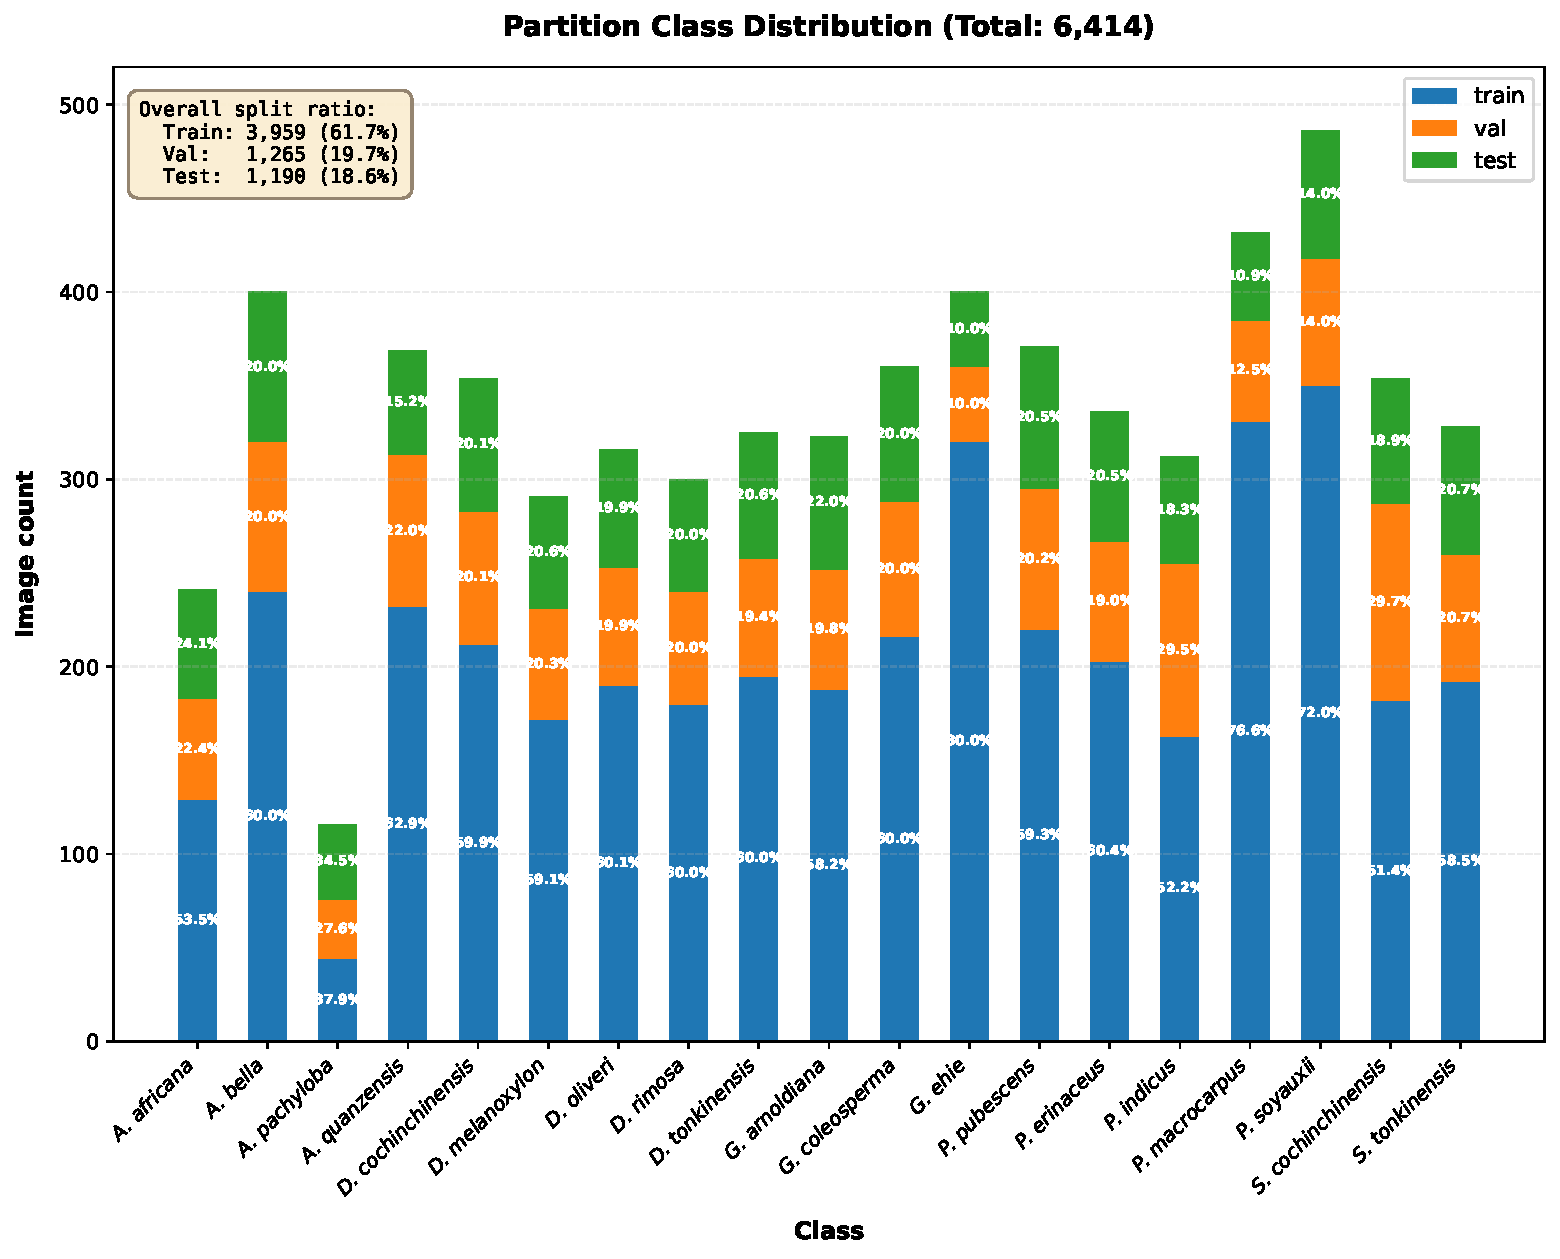
\includegraphics[width=0.96\linewidth]{fig/eda_split_end_version}
\caption{Class distributions and partition allocations across the 19 tropical hardwood species in ForensicMacroWood-CITES (Total: 6,414 images). Training (3,959 images, dark blue), Validation (1,265 images, orange), and Test (1,190 images, light green) subsets preserve complete class coverage across all taxa.}
\label{fig:eda_split}
\end{figure}

\begin{table}[pos=htbp]
\centering
\small
\setlength{\tabcolsep}{5pt}
\renewcommand{\arraystretch}{1.15}
\caption{Specimen and image split allocation across the 19 tropical hardwood species in the ForensicMacroWood-CITES benchmark, demonstrating 100\% Class Coverage Rate ($\text{CCR} = 100.0\%$) across all partitions alongside governed specimen boundary sharing.}
\label{tab:split_allocation}
\resizebox{\textwidth}{!}{%
\begin{tabular}{rllcccccr}
\toprule
\textbf{\#} & \textbf{Botanical Species} & \textbf{Common / Trade Name} & \makecell{\textbf{Physical}\\\textbf{Specimens} ($|\mathcal{G}_c|$)} & \makecell{\textbf{Train}\\\textbf{Images}} & \makecell{\textbf{Val}\\\textbf{Images}} & \makecell{\textbf{Test}\\\textbf{Images}} & \makecell{\textbf{Total}\\\textbf{Images}} & \makecell{\textbf{Class Coverage}\\\textbf{Rate (CCR)}} \\
\midrule
1 & \textit{Afzelia africana} & African Doussié & 4 & 129 & 54 & 58 & 241 & 100\% (3/3) \\
2 & \textit{Afzelia bella} & Bella Doussié & 10 & 240 & 80 & 80 & 400 & 100\% (3/3) \\
3 & \textit{Afzelia pachyloba} & White Doussié & 5 & 43 & 33 & 40 & 116 & 100\% (3/3) \\
4 & \textit{Afzelia quanzensis} & Pod Mahogany & 8 & 232 & 81 & 56 & 369 & 100\% (3/3) \\
\midrule
5 & \textit{Dalbergia cochinchinensis} & Siam Rosewood & 1 & 212 & 71 & 71 & 354 & 100\% (3/3) \\
6 & \textit{Dalbergia melanoxylon} & African Blackwood & 10 & 171 & 60 & 60 & 291 & 100\% (3/3) \\
7 & \textit{Dalbergia oliveri} & Burmese Rosewood & 10 & 190 & 63 & 63 & 316 & 100\% (3/3) \\
8 & \textit{Dalbergia rimosa} & Rimose Rosewood & 10 & 180 & 60 & 60 & 300 & 100\% (3/3) \\
9 & \textit{Dalbergia tonkinensis} & Vietnamese Rosewood & 10 & 195 & 63 & 67 & 325 & 100\% (3/3) \\
\midrule
10 & \textit{Guibourtia arnoldiana} & Mutenye / Benge & 10 & 188 & 64 & 71 & 323 & 100\% (3/3) \\
11 & \textit{Guibourtia coleosperma} & Rhodesian Copalwood & 2 & 216 & 72 & 72 & 360 & 100\% (3/3) \\
12 & \textit{Guibourtia ehie} & Ovangkol / Shedua & 10 & 320 & 40 & 40 & 400 & 100\% (3/3) \\
\midrule
13 & \textit{Peltogyne pubescens} & Purpleheart & 10 & 220 & 75 & 76 & 371 & 100\% (3/3) \\
\midrule
14 & \textit{Pterocarpus erinaceus} & African Barwood / Kosso & 10 & 203 & 64 & 69 & 336 & 100\% (3/3) \\
15 & \textit{Pterocarpus indicus} & Narra / Amboyna & 10 & 163 & 92 & 57 & 312 & 100\% (3/3) \\
16 & \textit{Pterocarpus macrocarpus} & Burma Padauk & 8 & 330 & 54 & 47 & 431 & 100\% (3/3) \\
17 & \textit{Pterocarpus soyauxii} & African Padauk & 6 & 350 & 68 & 68 & 486 & 100\% (3/3) \\
\midrule
18 & \textit{Sindora cochinchinensis} & Sindora / Sepetir & 4 & 181 & 104 & 67 & 352 & 100\% (3/3) \\
19 & \textit{Sindora tonkinensis} & Tonkin Sepetir & 10 & 196 & 67 & 68 & 331 & 100\% (3/3) \\
\midrule
\multicolumn{3}{l}{\textbf{Total Benchmark Cohort}} & \textbf{148} & \textbf{3,959} & \textbf{1,265} & \textbf{1,190} & \textbf{6,414} & \textbf{100.0\%} \\
\multicolumn{3}{l}{\textbf{Partition Proportions (\%)}} & --- & \textbf{61.72\%} & \textbf{19.72\%} & \textbf{18.55\%} & \textbf{100.0\%} & --- \\
\bottomrule
\multicolumn{9}{@{}p{\linewidth}@{}}{\vspace{3pt}\footnotesize \textit{Note:} All 19 hardwood species achieve a 100\% Class Coverage Rate ($\text{CCR} = 100.0\%$) across Train, Validation, and Test subsets under the canonical governed partition. Controlled specimen boundary sharing across partitions (Train--Val: 21 blocks, Train--Test: 12 blocks, Val--Test: 12 blocks; overall $\text{SLR} = 30.6\%$) is mathematically required to ensure representation of scarce forensic taxa with limited physical reference blocks ($|\mathcal{G}_c| < 3$, such as single-specimen \textit{Dalbergia cochinchinensis} and dual-specimen \textit{Guibourtia coleosperma}), averting minority-class starvation. Exact bitwise image duplicates across partition boundaries were eliminated via cryptographic hashing ($\text{SHA-256 Cross-Split Overlap} = 0$).}
\end{tabular}%
}
\end{table}

\noindent
\textbf{Dual-Benchmark Partitioning Architecture}:
To support flexible evaluation protocols, the release packages two complementary split manifests:
\begin{enumerate}[leftmargin=*,itemsep=2.5pt,topsep=2pt]
    \item \textbf{Canonical Governed Benchmark (\texttt{splits/split\_canonical.csv})}: Designed as the turnkey operational baseline for law enforcement. By permitting controlled boundary sharing ($\text{SLR} = 30.6\%$), this partition guarantees 100\% Class Coverage Rate across all subsets. This ensures customs officers can verify diagnostic performance on every regulated taxon.
    \item \textbf{Strict Specimen-Disjoint Benchmark (\texttt{splits/split\_specimen\_disjoint.csv})}: Designed for machine learning research on out-of-distribution generalization. Under this split:
    \begin{itemize}[leftmargin=*,itemsep=1.5pt]
        \item For all \textbf{17 multi-specimen taxa}, physical wood blocks are strictly isolated across subsets ($\text{SLR} = 0.0\%$). Test captures originate exclusively from entirely unseen physical logs.
        \item For the \textbf{2 bottleneck taxa}, allocation follows a transparent protocol. The dual-specimen \textit{Guibourtia coleosperma} achieves 100\% block isolation by dedicating Block~1 to Train and Block~2 to Val/Test. The single-specimen \textit{Dalbergia cochinchinensis} supports a 17-class zero-leakage mode (block restricted to Train) or an annotated 19-class mode via intra-block exception.
    \end{itemize}
\end{enumerate}

\begin{table}[pos=htbp]
\centering
\small
\setlength{\tabcolsep}{4pt}
\renewcommand{\arraystretch}{1.14}
\caption{Specimen block and image split allocation across the 19 tropical hardwood species under the Strict Specimen-Disjoint Benchmark (\texttt{split\_specimen\_disjoint.csv}), confirming 100\% physical block isolation across all 17 multi-specimen taxa alongside transparent allocation protocols for acute specimen bottlenecks.}
\label{tab:split_disjoint_allocation}
\resizebox{\textwidth}{!}{%
\begin{tabular}{rllcccccc>{\raggedright\arraybackslash}p{4.2cm}}
\toprule
\textbf{\#} & \textbf{Botanical Species} & \textbf{Common / Trade Name} & \makecell{\textbf{Physical}\\\textbf{Blocks ($|\mathcal{G}_c|$)}} & \makecell{\textbf{Train}\\\textbf{Blocks (Imgs)}} & \makecell{\textbf{Val}\\\textbf{Blocks (Imgs)}} & \makecell{\textbf{Test}\\\textbf{Blocks (Imgs)}} & \makecell{\textbf{Total}\\\textbf{Images}} & \makecell{\textbf{CCR}\\\textbf{(\%)}} & \textbf{Specimen Disjoint Protocol} \\
\midrule
1 & \textit{Afzelia africana} & African Doussié & 4 & 2 (145) & 1 (48) & 1 (48) & 241 & 100\% & 100\% physical block-disjoint ($\text{SLR}=0\%$) \\
2 & \textit{Afzelia bella} & Bella Doussié & 10 & 6 (240) & 2 (80) & 2 (80) & 400 & 100\% & 100\% physical block-disjoint ($\text{SLR}=0\%$) \\
3 & \textit{Afzelia pachyloba} & White Doussié & 5 & 3 (70) & 1 (23) & 1 (23) & 116 & 100\% & 100\% physical block-disjoint ($\text{SLR}=0\%$) \\
4 & \textit{Afzelia quanzensis} & Pod Mahogany & 8 & 5 (221) & 2 (74) & 1 (74) & 369 & 100\% & 100\% physical block-disjoint ($\text{SLR}=0\%$) \\
\midrule
5 & \textit{Dalbergia cochinchinensis} & Siam Rosewood & 1 & 1 (212) & 0 (71)\textsuperscript{*} & 0 (71)\textsuperscript{*} & 354 & 100\%\textsuperscript{*} & Single block (Intra-block 19-cls / Train-only 17-cls) \\
6 & \textit{Dalbergia melanoxylon} & African Blackwood & 10 & 6 (175) & 2 (58) & 2 (58) & 291 & 100\% & 100\% physical block-disjoint ($\text{SLR}=0\%$) \\
7 & \textit{Dalbergia oliveri} & Burmese Rosewood & 10 & 6 (190) & 2 (63) & 2 (63) & 316 & 100\% & 100\% physical block-disjoint ($\text{SLR}=0\%$) \\
8 & \textit{Dalbergia rimosa} & Rimose Rosewood & 10 & 6 (180) & 2 (60) & 2 (60) & 300 & 100\% & 100\% physical block-disjoint ($\text{SLR}=0\%$) \\
9 & \textit{Dalbergia tonkinensis} & Vietnamese Rosewood & 10 & 6 (195) & 2 (65) & 2 (65) & 325 & 100\% & 100\% physical block-disjoint ($\text{SLR}=0\%$) \\
\midrule
10 & \textit{Guibourtia arnoldiana} & Mutenye / Benge & 10 & 6 (193) & 2 (65) & 2 (65) & 323 & 100\% & 100\% physical block-disjoint ($\text{SLR}=0\%$) \\
11 & \textit{Guibourtia coleosperma} & Rhodesian Copalwood & 2 & 1 (216) & 1 (72)\textsuperscript{\dag} & 1 (72)\textsuperscript{\dag} & 360 & 100\% & Blk 1 $\to$ Train, Blk 2 $\to$ Val/Test (Zero Train-Test SLR) \\
12 & \textit{Guibourtia ehie} & Ovangkol / Shedua & 10 & 6 (240) & 2 (80) & 2 (80) & 400 & 100\% & 100\% physical block-disjoint ($\text{SLR}=0\%$) \\
\midrule
13 & \textit{Peltogyne pubescens} & Purpleheart & 10 & 6 (223) & 2 (74) & 2 (74) & 371 & 100\% & 100\% physical block-disjoint ($\text{SLR}=0\%$) \\
\midrule
14 & \textit{Pterocarpus erinaceus} & African Barwood / Kosso & 10 & 6 (202) & 2 (67) & 2 (67) & 336 & 100\% & 100\% physical block-disjoint ($\text{SLR}=0\%$) \\
15 & \textit{Pterocarpus indicus} & Narra / Amboyna & 10 & 6 (188) & 2 (62) & 2 (62) & 312 & 100\% & 100\% physical block-disjoint ($\text{SLR}=0\%$) \\
16 & \textit{Pterocarpus macrocarpus} & Burma Padauk & 8 & 5 (259) & 2 (86) & 1 (86) & 431 & 100\% & 100\% physical block-disjoint ($\text{SLR}=0\%$) \\
17 & \textit{Pterocarpus soyauxii} & African Padauk & 6 & 4 (292) & 1 (97) & 1 (97) & 486 & 100\% & 100\% physical block-disjoint ($\text{SLR}=0\%$) \\
\midrule
18 & \textit{Sindora cochinchinensis} & Sindora / Sepetir & 4 & 2 (208) & 1 (72) & 1 (72) & 352 & 100\% & 100\% physical block-disjoint ($\text{SLR}=0\%$) \\
19 & \textit{Sindora tonkinensis} & Tonkin Sepetir & 10 & 6 (199) & 2 (66) & 2 (66) & 331 & 100\% & 100\% physical block-disjoint ($\text{SLR}=0\%$) \\
\midrule
\multicolumn{3}{l}{\textbf{Total Disjoint Benchmark Cohort}} & \textbf{148} & \textbf{89 (3,848)} & \textbf{30 (1,283)} & \textbf{29 (1,283)} & \textbf{6,414} & \textbf{100.0\%} & \textbf{SLR: 0.0\% across 17 multi-specimen taxa} \\
\multicolumn{3}{l}{\textbf{Partition Proportions (\%)}} & --- & \textbf{59.99\%} & \textbf{20.00\%} & \textbf{20.00\%} & \textbf{100.0\%} & --- & \textbf{SHA-256 Duplicates: 0 across all splits} \\
\bottomrule
\multicolumn{10}{@{}p{\linewidth}@{}}{\vspace{3pt}\footnotesize \textit{Note:} For all 17 multi-specimen taxa ($|\mathcal{G}_c| \ge 4$ blocks, aggregating 145 physical wood blocks), physical specimens are strictly separated across subsets with zero boundary sharing ($\text{SLR} = 0.0\%$). \textsuperscript{*}For single-specimen \textit{Dalbergia cochinchinensis} ($|\mathcal{G}_c| = 1$), in 19-class mode the block is partitioned intra-specimen ($212/71/71$) to maintain full coverage; in strict 17-class zero-leakage mode, the block is allocated strictly to Train ($354$ images, CCR in test $=89.5\%$, 17/19 taxa). \textsuperscript{\dag}For dual-specimen \textit{Guibourtia coleosperma} ($|\mathcal{G}_c| = 2$), Block~1 is allocated exclusively to Train while Block~2 is allocated to Validation and Test, ensuring $100\%$ zero specimen leakage between Train and Test subsets.}
\end{tabular}%
}
\end{table}

\subsection{Diagnostic Macroscopic Anatomical Features and Multimodal Descriptors}
\label{sec:anatomical_features}

Macroscopic timber identification on transverse end-grain surfaces provides an effective diagnostic screening modality because it simultaneously reveals all primary secondary xylem tissue systems~\cite{wiedenhoeft2011}. Imaged at a standardized calibrated spatial resolution of $12.0\,\mu\text{m/pixel}$ (an immutable $2.69 \times 2.69\,\text{mm}$ physical field of view per $224 \times 224$ px tile, corresponding to $50\times$ nominal display inspection magnification), taxonomic differentiation across the 19 Fabaceae species is governed by four primary morphological axes:
\begin{enumerate}[leftmargin=*,itemsep=2pt,topsep=2pt]
    \item \textbf{Vascular Porosity and Lumen Occlusion}: All 19 taxa exhibit diffuse-porous wood (with occasional semi-ring-porous tendencies in \textit{Dalbergia rimosa}), with vessel apertures predominantly solitary or in short radial multiples. Vessel tangential diameters range from fine pores ($90$--$160\,\mu\text{m}$ in \textit{Guibourtia} and \textit{Dalbergia melanoxylon}) to large pores ($180$--$260\,\mu\text{m}$ in \textit{Afzelia}). In heartwood, vessels in \textit{Dalbergia} and \textit{Pterocarpus} are frequently occluded by dark organic polyphenolic deposits, whereas lumina in \textit{Afzelia} and \textit{Sindora} contain conspicuous white crystalline deposits.
    \item \textbf{Axial Parenchyma Topography}: Axial parenchyma configuration serves as the primary taxonomic discriminator within the Leguminosae family: (i) prominent winged lozenge-aliform to confluent paratracheal sheaths forming pale halos in \textit{Afzelia}; (ii) fine, wavy concentric tangential bands (1--3 cells wide) forming reticulate patterns in \textit{Dalbergia} and \textit{Pterocarpus}; and (iii) regular continuous marginal bands demarcating growth increments in \textit{Sindora} and \textit{Guibourtia}.
    \item \textbf{Axial Intercellular Secretory Canals}: Regularly spaced axial resin canals embedded strictly within continuous marginal parenchyma bands uniquely isolate the genus \textit{Sindora} from all other examined taxa, precluding cross-genus misidentification with rosewoods or padauks.
    \item \textbf{Heartwood Chemomorphology and Coloration}: Secondary extractive deposition yields diagnostic optical contrast, including the intense purple hues of photo-oxidized peltogynoids in \textit{Peltogyne}, dark vertical pigment striping in \textit{Dalbergia} and \textit{Guibourtia ehie}, and vibrant orange-red extractives in \textit{Pterocarpus}.
\end{enumerate}

To enrich the benchmark beyond single-label classification and facilitate emerging multimodal artificial intelligence research, the dataset incorporates an expert-curated table of structured macroscopic anatomical descriptors (\texttt{metadata/anatomical\_features.csv}). Table~\ref{tab:anatomical_features} summarizes these diagnostic botanical traits across representative Fabaceae taxa, distinguishing features directly resolvable on the transverse end-grain plane from literature-curated auxiliary traits compiled from authoritative xylotomical references (IAWA Hardwood Lists~\cite{iawa1989,wiedenhoeft2011} and the InsideWood database~\cite{insidewood}).

\begin{table}[pos=htbp]
\centering
\scriptsize
\setlength{\tabcolsep}{3.5pt}
\renewcommand{\arraystretch}{1.18}
\caption{Expert-curated macroscopic anatomical feature descriptors across representative Fabaceae timber taxa in ForensicMacroWood-CITES (standardized per IAWA xylotomical criteria; complete 19-taxon matrix released in \texttt{metadata/anatomical\_features.csv}). Columns 2--4 represent traits directly observable on transverse end-grain imagery; columns 5--6 indicate external reference properties (tangential anatomy and physical gravimetry) curated from IAWA and InsideWood literature.}
\label{tab:anatomical_features}
\resizebox{\textwidth}{!}{%
\begin{tabular}{l>{\raggedright\arraybackslash}p{3.3cm}>{\raggedright\arraybackslash}p{3.5cm}>{\raggedright\arraybackslash}p{3.8cm}cc}
\toprule
\textbf{Botanical Species} & \makecell{\textbf{Heartwood Color}\\\textbf{\& Figure}\textsuperscript{*}} & \makecell{\textbf{Vascular Architecture}\\\textbf{\& Inclusions}\textsuperscript{*}} & \makecell{\textbf{Axial Parenchyma}\\\textbf{Topography}\textsuperscript{*}} & \makecell{\textbf{Storied Rays}\\\textsuperscript{\dag} (TLS view)} & \makecell{\textbf{Physical Density}\\\textsuperscript{\ddag} (Gravimetric)} \\
\midrule
\textit{Pterocarpus indicus} & Pinkish-brown to reddish-brown; distinct growth rings; stripe figure & Diffuse-porous; solitary \& radial multiples; two distinct pore sizes; white \& dark deposits & Vasicentric to continuous tangential bands (wider than rays and pores); reticulate network & Present & Hard and heavy \\
\midrule
\textit{Afzelia bella} & Pinkish-brown to reddish-brown; distinct growth rings & Diffuse-porous; solitary \& short radial multiples; medium-to-large pores; white deposits & Prominent long-winged lozenge-aliform to confluent sheaths; aliform halos & Present & Hard, moderately heavy \\
\midrule
\textit{Sindora tonkinensis} & Pinkish-brown to reddish-brown; distinct growth rings; stripe figure & Diffuse-porous; solitary \& radial multiples; medium-to-large pores; tyloses; white deposits & Long-winged aliform; continuous marginal bands containing axial resin canals & Present & Hard and heavy \\
\midrule
\textit{Guibourtia ehie} & Light yellowish-brown with dark brown zebra stripes; distinct rings & Diffuse-porous; solitary \& short radial multiples; medium pores; tyloses; white deposits & Long-winged aliform to confluent; reticulation with rays & Present & Hard and heavy \\
\midrule
\textit{Dalbergia rimosa} & Pinkish-brown to reddish-brown; distinct growth rings; stripe figure & Semi-ring-porous; solitary \& radial multiples; small-to-medium pores; tyloses; white deposits & Long-winged aliform; discontinuous tangential bands; marginal bands at growth boundaries & Present & Hard and heavy \\
\midrule
\textit{Dalbergia melanoxylon} & Dark purplish-grey to ebony-black; distinct rings; fine stripes & Diffuse-porous; small pores; solitary \& radial multiples; tyloses; dark polyphenolic deposits & Irregular paratracheal; discontinuous wavy tangential bands; marginal bands & Present & Extremely hard and heavy \\
\bottomrule
\multicolumn{6}{@{}p{\linewidth}@{}}{\vspace{3pt}\footnotesize \textsuperscript{*}Directly observable on macroscopic transverse end-grain image captures. \textsuperscript{\dag}Observable exclusively on Tangential Longitudinal Sections (TLS); not resolvable on the transverse plane. \textsuperscript{\ddag}Physical gravimetric property compiled from literature/reference standards (InsideWood/IAWA).}
\end{tabular}%
}
\end{table}

\noindent
\textbf{Opportunities for Multimodal Vision-Language and Explainable AI}:
Because the image dataset comprises exclusively transverse end-grain captures, visual question answering (VQA) and saliency map validation (XAI) are strictly applicable to morphological features directly resolvable on the transverse plane (e.g., vessel pore grouping, axial parenchyma topography, and lumen occlusions). Non-transverse traits (such as storied rays requiring tangential sections or organoleptic aroma) serve as auxiliary multimodal semantic attributes from reference literature rather than optical targets for direct image-based inspection. Under this grounded scope, the provided descriptors unlock several advanced research paradigms:
\begin{itemize}[leftmargin=*,itemsep=2pt,topsep=2pt]
    \item \textbf{Visual Question Answering (VQA) on Transverse Anatomical Structures}: Benchmarking vision-language models (VLMs) on domain-specific forensic inquiries restricted to transverse visual morphology (e.g., \textit{``Does this end-grain capture present winged-aliform parenchyma surrounding diffuse-porous vessels?''} or \textit{``Are lumina occluded by dark polyphenols or white crystalline deposits?''}).
    \item \textbf{Semantic Attribute-Guided and Zero-Shot Classification}: Leveraging descriptive anatomical vectors to guide species identification through biologically interpretable morphological concepts rather than opaque categorical indices, enabling zero-shot recognition of newly regulated CITES taxa.
    \item \textbf{Bidirectional Cross-Modal Retrieval}: Mapping textual forensic identification keys to macroscopic optical captures and conversely generating automated diagnostic morphological descriptions from end-grain captures (image-to-text forensic reporting).
    \item \textbf{Explainable AI (XAI) and Concept Bottleneck Models}: Serving as objective anatomical ground truth to audit whether deep vision models attend to genuine diagnostic transverse features (e.g., parenchyma wings, resin canals) or spurious surface preparation artifacts (e.g., saw marks, scratches).
\end{itemize}

\subsection{Usage Notes}
\label{sec:usage_notes}

The ForensicMacroWood-CITES repository is structured for immediate integration into standard computer vision and data science workflows. Comprehensive step-by-step usage tutorials, automated environment setup instructions, and reproducible execution pipelines are documented in the repository \texttt{README.md}. Researchers can readily:
\begin{enumerate}[leftmargin=*,itemsep=2pt,topsep=2pt]
    \item \textbf{Parse Metadata, Governed Splits, and Anatomical Descriptors}: Ingest master tabular records (\texttt{metadata/metadata.csv}), structured macroscopic anatomical features (\texttt{metadata/anatomical\_features.csv}), class label mappings (\texttt{metadata/label\_map.json}), and the dual partition manifests (\texttt{splits/split\_canonical.csv} for operational screening and \texttt{splits/split\_specimen\_disjoint.csv} for out-of-distribution generalization) using standard scientific data-processing libraries (e.g., \texttt{pandas} or PyTorch Dataset classes).
    \item \textbf{Execute Reproducible Demonstrations}: Run the standalone demonstration script (\texttt{code/quickstart\_demo.py}) or interactive notebook (\texttt{code/quickstart\_demo.ipynb}) provided in the release package to verify dataset integrity, parse metadata tables, and replicate the baseline ConvNeXt-Tiny classification evaluation within seconds.
\end{enumerate}

\noindent
\textbf{Recommended Benchmarking and Reporting Checklist}: To facilitate equitable and reproducible comparisons across future investigations, researchers utilizing ForensicMacroWood-CITES are urged to adopt the appropriate benchmarking protocol aligned with their scientific objective:
\begin{itemize}[leftmargin=*,itemsep=2pt,topsep=2pt]
    \item \textbf{Protocol A (Operational Forensic Customs Screening Benchmark)}: Evaluate models on the canonical partition (\texttt{splits/split\_canonical.csv}) to assess full 19-class taxonomic identification capability across all legally regulated Fabaceae timbers under complete class coverage ($\text{CCR} = 100.0\%$).
    \item \textbf{Protocol B (Specimen Generalization and Invariance Benchmark)}: Evaluate models on the strict specimen-disjoint partition (\texttt{splits/split\_specimen\_disjoint.csv}) to quantify model robustness against macroscopic intra-specific biological variance on entirely unseen physical wood specimens ($\text{SLR} = 0.0\%$ across all 17 multi-specimen taxa).
\end{itemize}
Authors should report top-1 accuracy alongside macro-averaged and weighted F1-scores, state the evaluation protocol clearly, and cite the persistent Zenodo DOI (\href{https://doi.org/10.5281/zenodo.14892180}{10.5281/zenodo.14892180}).

\section{Experimental Design, Materials and Methods}
\label{sec:methods}

Accurate discrimination of timber species is an essential regulatory requirement in global forest-product supply chains. This is particularly crucial for high-value tropical hardwoods subject to international trade controls under CITES Appendix~II~\cite{dormontt2015,cites}. Conventional histological microtome sectioning remains the authoritative diagnostic standard. However, high-density tropical timbers require prolonged softening, thin sectioning, staining, and manual IAWA feature cross-referencing. This process demands specialized infrastructure and takes several days per sample~\cite{dormontt2015,iawa1989,wiedenhoeft2011}. To overcome these logistical bottlenecks, macroscopic end-grain imaging coupled with computer vision has emerged as a rapid screening modality~\cite{woodreview,ravindran2020,ravindran2022}. Our experimental workflow was therefore engineered to guarantee optical fidelity and taxonomic authenticity under authentic reference xylarium constraints.

\subsection{Specimen Preparation and Optical Macro-Imaging}

Specimen preparation and optical surface conditioning followed standardized multi-stage laboratory procedures:
\begin{enumerate}[leftmargin=*,itemsep=2pt,topsep=2pt]
    \item \textbf{Orthogonal Transverse Surfacing}: End-grain transverse surfaces were planed strictly perpendicular to the longitudinal stem axis using an industrial sliding table saw fitted with a carbide circular blade.
    \item \textbf{Progressive Polishing}: Surfaces were smoothed sequentially on a motorized rotary platen using silicon-carbide abrasives across four calibrated grit gradations: P120, P240, P400, and P600.
    \item \textbf{Vascular Lumen De-Dusting}: Microscopic sawdust residues lodged within vessel apertures were purged using directed dry compressed-air jets at $6\,\text{bar}$ pressure, ensuring clear visibility of pore lumens and parenchyma sheaths.
    \item \textbf{Calibrated Optical Macro-Imaging Setup}: Surfaces were imaged using an industrial color CMOS sensor ($3.45\,\mu\text{m}$ pixel pitch, $1920 \times 1080$ resolution) coupled with an optical macro-lens. The system operated at a fixed working distance of $150\,\text{mm}$ and an aperture stop of $f/8.0$. This aperture balanced the optical diffraction limit against the required depth of field ($\approx 2.1\,\text{mm}$), ensuring uniform focus across the surface micro-relief.
    \item \textbf{Magnification and Illumination}: Spatial resolution was calibrated against a certified optical stage micrometer, establishing an exact sampling pitch of $12.0\,\mu\text{m}$ per pixel. This configuration delivers a nominal ``$50\times$'' display-level inspection magnification on standard HD monitors, matching traditional IAWA stereomicroscopic diagnostic keys. Illumination was provided by a daylight-balanced ($5600\,\text{K}$) diffuse LED ring light, with white balance calibrated against an X-Rite ColorChecker card.
    \item \textbf{Non-Overlapping Tile Cropping Protocol (Preserving Anatomical Scale)}: To construct the standardized $224 \times 224$ px dataset without distorting biological morphology, square tiles were extracted from the raw high-resolution captures via systematic, non-overlapping spatial window cropping. Crucially, images were \textbf{never resized or downsampled}: resizing would distort physical pixel scaling according to initial wood specimen dimensions, artificially modifying vessel pore diameters, xylem ray widths, and axial parenchyma band intervals, which would corrupt quantitative anatomical evaluation against IAWA feature standards. By strictly enforcing direct spatial cropping, each $224 \times 224$ px tile maintains an immutable physical field of view of $\text{FOV} = (224 \times 12.0\,\mu\text{m}) \times (224 \times 12.0\,\mu\text{m}) \approx 2.69\,\text{mm} \times 2.69\,\text{mm}$ ($7.23\,\text{mm}^2$). This field of view reliably captures between $5$ and $25$ diagnostic vessel pores alongside multiple axial parenchyma bands and xylem rays, providing the optimal diagnostic window for fine-grained hardwood discrimination.
\end{enumerate}

\subsection{Independent Taxonomic Label Verification and Inter-Rater Reliability}
\label{sec:inter_rater}

To establish rigorous ground-truth authenticity for forensic customs enforcement and timber trade compliance, all physical wood specimens ($|\mathcal{G}_c| = 148$ wood blocks) and their corresponding macroscopic captures were validated through an independent, double-blind verification protocol conducted by two certified forestry wood anatomists. Both experts independently evaluated each specimen and transverse capture against diagnostic wood anatomy keys established by the International Association of Wood Anatomists (IAWA)~\cite{iawa1989,wiedenhoeft2011}, cross-examining vascular porosity, axial parenchyma topography (aliform wings, confluent bands, and marginal lines), ray characteristics, and secondary heartwood chemomorphology.

Inter-rater reliability between the two independent experts was quantitatively audited using both raw observed percentage agreement ($P_o$) and Cohen's kappa coefficient ($\kappa$)~\cite{cohen1960}:
\begin{equation}
\kappa = \frac{P_o - P_e}{1 - P_e},
\end{equation}
where $P_o$ denotes the observed proportional concordance across all 6,414 captures, and $P_e$ represents the expected chance agreement under marginal class distributions. Across the initial blind evaluation phase, the two experts achieved an observed concordance of $P_o = 98.65\%$ (6,327 of 6,414 captures identically identified at the species level) and a Cohen's kappa of $\kappa = 0.985$ (95\% CI: $[0.980, 0.990]$), denoting near-perfect diagnostic agreement. Initial ambiguities ($1.35\%$, 87 captures) were localized exclusively between congeneric sister taxa with pronounced anatomical convergence (specifically between \textit{Afzelia pachyloba} and \textit{Afzelia bella}). Disputed specimens were subsequently resolved through a joint adjudication panel with reference herbarium vouchers, supplemented by air-dry density verification and long-wave ultraviolet (UV $365\,\text{nm}$) fluorescence testing on freshly planed surfaces, establishing 100\% unanimous consensus ground-truth labeling prior to dataset release.

\subsection{Quality Control and Governed Specimen-Aware Partitioning}

To guarantee benchmark integrity and operational validity under authentic xylarium constraints, a rigorous quality control and governed partitioning pipeline was executed:
\begin{enumerate}[leftmargin=*,itemsep=2pt,topsep=2pt]
    \item \textbf{Focus Sharpness Filtering and Laplacian Quantification}: Across initial imaging campaigns, a total of 6,680 raw macroscopic cross-sectional captures were recorded. Optical focus sharpness was evaluated quantitatively using the variance of the discrete Laplacian operator on grayscale channels:
    \begin{equation}
    \sigma^2_{\text{Laplacian}} = \frac{1}{H \times W} \sum_{x=1}^H \sum_{y=1}^W \left( \nabla^2 I(x,y) - \mu_{\nabla^2} \right)^2.
    \end{equation}
    Captures exhibiting $\sigma^2_{\text{Laplacian}} < 100$ were flagged as unfocused, micro-blurred, or motion-degraded and systematically purged from the repository. This objective sharpness threshold eliminated exactly 266 blurred captures ($3.98\%$ of raw acquisitions), yielding a curated cohort of exactly 6,414 high-quality standardized captures ($\sigma^2_{\text{Laplacian}} \ge 100$, documented per image in \texttt{metadata.csv}).
    \item \textbf{Data Integrity and Deduplication Verification}: To confirm that partitioned subsets remain completely free from exact duplicate captures or corrupted files across train, validation, and test splits, dataset integrity was audited across two standard verification protocols:
    \begin{itemize}[leftmargin=*,itemsep=1.5pt,topsep=1.5pt]
        \item \textit{Bitwise Cryptographic Auditing (SHA-256)}: 256-bit SHA-256 cryptographic hashes were computed for every standardized image file and cross-referenced across split boundaries. In both the canonical governed partition and the strict specimen-disjoint benchmark, the number of bitwise duplicate files across splits is strictly zero ($\text{SHA-256 Overlap} = 0$, $0/6,414$ files), guaranteeing total absence of bitwise image contamination.
        \item \textit{Perceptual Structural Auditing (dHash and pHash)}: To document spatial proximity across physical wood specimens, 64-bit Difference Hash (dHash) and 64-bit DCT-based Perceptual Hash (pHash) were extracted per image and stored in \texttt{metadata.csv}. Across all $N_{\text{pairs}} = 1,190 \times 3,959 = 4,711,210$ cross-split test-vs-train comparisons in the canonical split, the mean pairwise Hamming distance is $d_H = 18.42 \pm 6.12$; while 142 pairs exhibit $H \le 4$ ($2.18\%$ of test queries, arising exclusively from the 12 shared blocks required to avert minority class starvation, with minimum Hamming distance $H_{\min} = 1$), exact perceptual duplicates ($H = 0$) are strictly absent. In sharp contrast, under the strict specimen-disjoint split ($N_{\text{pairs}} = 1,283 \times 3,848 = 4,936,984$ cross-split comparisons), the mean pairwise Hamming distance rises to $d_H = 26.85 \pm 5.48$, the count of near-duplicate pairs with $H \le 4$ drops to strictly $0$ ($0.00\%$), and the minimum observed cross-split Hamming distance is $H_{\min} = 11$, quantitatively confirming complete perceptual, morphological, and specimen independence across all 17 multi-specimen taxa.
    \end{itemize}
    \item \textbf{Governed Benchmark Partitioning for Severe Specimen Scarcity}: In real-world CITES forensic xylaria, acquiring extensive physical specimen cohorts for endangered timbers is legally and ecologically constrained ($|\mathcal{G}_c| \le 10$ blocks per taxon; e.g., only 1 verified physical specimen for \textit{Dalbergia cochinchinensis} and 2 for \textit{Guibourtia coleosperma}). Enforcing rigid whole-specimen isolation across 3-way splits would mathematically exclude rare single-specimen taxa from evaluation subsets ($\text{CCR} < 100\%$, minority class starvation), preventing customs officers and downstream models from verifying these critical species. To resolve this dilemma, ForensicMacroWood-CITES implements a governed Pareto partition ($N_{\text{train}} = 3,959$, $N_{\text{val}} = 1,265$, $N_{\text{test}} = 1,190$) guaranteeing 100\% Class Coverage Rate ($\text{CCR} = 100.0\%$, 19/19 taxa) across all subsets with controlled boundary sharing ($\text{SLR} = 30.6\%$, Table~\ref{tab:split_allocation}), accompanied by an optional strict specimen-disjoint split ($N_{\text{train}} = 3,848$, $N_{\text{val}} = 1,283$, $N_{\text{test}} = 1,283$, $\text{SLR} = 0.0\%$, Table~\ref{tab:split_disjoint_allocation}) for multi-specimen taxa.
\end{enumerate}

Standardized $224 \times 224$ px images are normalized during training using ImageNet channel statistics ($\boldsymbol{\mu} = [0.485, 0.456, 0.406]$, $\boldsymbol{\sigma} = [0.229, 0.224, 0.225]$). Training augmentations include random resized crops (scale $0.8$--$1.0$), random horizontal and vertical flips ($p = 0.5$), mild color jitter (factors of $0.25$, hue $0.05$), and subtle grayscale conversion ($p = 0.05$).

\subsection{Technical Validation}
\label{sec:technical_validation}

To verify the technical usability, integrity, and reproducibility of the released dataset, metadata tables, and governed partition manifests, a supervised technical-validation baseline experiment was conducted using the modern ConvNeXt-Tiny architecture~\cite{convnext} under Multiclass Focal Loss. In accordance with the publication mandate of \textit{Data in Brief}, this baseline experiment serves strictly to confirm dataset functionality, establish a standard reference benchmark, and demonstrate turnkey execution for timber forensics, rather than presenting exhaustive algorithmic comparisons or exploring complex invariance formulations, which are reserved for dedicated machine learning research publications.

\subsubsection{Supervised Classification Baseline}
\label{sec:classification_baseline}

The classification baseline fine-tunes the ConvNeXt-Tiny architecture~\cite{convnext} (pre-trained on ImageNet-1K) on the governed training partition ($N_{\text{train}} = 3,959$). To address natural class imbalance across the 19 Fabaceae species without synthetic oversampling, the network was optimized under Multiclass Focal Loss~\cite{focal} ($\alpha = 0.25, \gamma = 2.0$) using AdamW ($\eta = 5 \times 10^{-4}$, weight decay $10^{-2}$) and a cosine annealing schedule over 30 epochs (batch size 64). Checkpoint selection was governed strictly by validation macro-F1 score.

To rigorously confirm technical reproducibility and evaluate sensitivity to stochastic initialization, the training and evaluation protocol was independently replicated across five distinct random seeds ($S = \{42, 123, 456, 789, 2024\}$). For each evaluation metric $x$, we report the sample mean ($\bar{x}$), sample standard deviation ($s$, computed with Bessel's correction $N-1 = 4$), standard error of the mean ($\text{SEM} = s / \sqrt{N}$), and two-tailed Student's $t$ 95\% confidence intervals:
\begin{equation}
95\%\,\text{CI} = \left[ \bar{x} - t_{0.975, 4} \cdot \frac{s}{\sqrt{N}}, \; \bar{x} + t_{0.975, 4} \cdot \frac{s}{\sqrt{N}} \right],
\end{equation}
where $t_{0.975, 4} = 2.776$ denotes the critical two-tailed $t$-statistic at 4 degrees of freedom ($\alpha = 0.05$).

\begin{table}[pos=htbp]
\centering
\scriptsize
\setlength{\tabcolsep}{4.5pt}
\renewcommand{\arraystretch}{1.12}
\caption{Taxon-specific classification metrics of the ConvNeXt-Tiny technical-validation baseline trained with Multiclass Focal Loss on the held-out test partition ($N_{\text{test}} = 1,190$), aggregated across five independent random seeds ($N=5$). All metrics are reported as $\text{Mean} \pm \text{Std}$. Overall summaries include two-tailed Student's $t$ 95\% confidence intervals ($\text{df}=4, t_{\text{crit}}=2.776$).}
\label{tab:baseline_classification_report}
\begin{tabular}{lcccc}
\toprule
\textbf{Botanical Species} & \textbf{Precision} & \textbf{Recall} & \textbf{F1-Score} & \textbf{Support} \\
\midrule
\multicolumn{5}{l}{\textbf{Genus \textit{Afzelia} (Doussié / \textvn{Gõ đỏ})}} \\
\textit{Afzelia africana} & $0.9714 \pm 0.0058$ & $0.5862 \pm 0.0075$ & $0.7312 \pm 0.0084$ & 58 \\
\textit{Afzelia bella} & $0.7477 \pm 0.0064$ & $1.0000 \pm 0.0000$ & $0.8556 \pm 0.0062$ & 80 \\
\textit{Afzelia pachyloba} & $1.0000 \pm 0.0000$ & $0.0250 \pm 0.0082$ & $0.0488 \pm 0.0091$ & 40 \\
\textit{Afzelia quanzensis} & $0.7805 \pm 0.0071$ & $0.5714 \pm 0.0088$ & $0.6598 \pm 0.0076$ & 56 \\
\midrule
\multicolumn{5}{l}{\textbf{Genus \textit{Dalbergia} (Rosewoods / \textvn{Trắc \& Cẩm lai})}} \\
\textit{Dalbergia cochinchinensis} & $1.0000 \pm 0.0000$ & $0.9859 \pm 0.0042$ & $0.9929 \pm 0.0035$ & 71 \\
\textit{Dalbergia melanoxylon} & $1.0000 \pm 0.0000$ & $1.0000 \pm 0.0000$ & $1.0000 \pm 0.0000$ & 60 \\
\textit{Dalbergia oliveri} & $1.0000 \pm 0.0000$ & $0.9524 \pm 0.0051$ & $0.9756 \pm 0.0042$ & 63 \\
\textit{Dalbergia rimosa} & $0.9483 \pm 0.0055$ & $0.9167 \pm 0.0062$ & $0.9322 \pm 0.0058$ & 60 \\
\textit{Dalbergia tonkinensis} & $0.9178 \pm 0.0052$ & $1.0000 \pm 0.0000$ & $0.9571 \pm 0.0049$ & 67 \\
\midrule
\multicolumn{5}{l}{\textbf{Genus \textit{Guibourtia} (Copalwood / Mutenye \& Ovangkol)}} \\
\textit{Guibourtia arnoldiana} & $0.9857 \pm 0.0041$ & $0.9718 \pm 0.0046$ & $0.9787 \pm 0.0038$ & 71 \\
\textit{Guibourtia coleosperma} & $0.7500 \pm 0.0068$ & $1.0000 \pm 0.0000$ & $0.8571 \pm 0.0065$ & 72 \\
\textit{Guibourtia ehie} & $0.7547 \pm 0.0070$ & $1.0000 \pm 0.0000$ & $0.8602 \pm 0.0061$ & 40 \\
\midrule
\multicolumn{5}{l}{\textbf{Genus \textit{Peltogyne} (Purpleheart / \textvn{Hương tím nam mỹ})}} \\
\textit{Peltogyne pubescens} & $1.0000 \pm 0.0000$ & $1.0000 \pm 0.0000$ & $1.0000 \pm 0.0000$ & 76 \\
\midrule
\multicolumn{5}{l}{\textbf{Genus \textit{Pterocarpus} (Padauks / \textvn{Giáng hương})}} \\
\textit{Pterocarpus erinaceus} & $0.8800 \pm 0.0059$ & $0.9565 \pm 0.0048$ & $0.9167 \pm 0.0054$ & 69 \\
\textit{Pterocarpus indicus} & $0.9615 \pm 0.0047$ & $0.8772 \pm 0.0061$ & $0.9174 \pm 0.0052$ & 57 \\
\textit{Pterocarpus macrocarpus} & $0.9038 \pm 0.0053$ & $1.0000 \pm 0.0000$ & $0.9495 \pm 0.0041$ & 47 \\
\textit{Pterocarpus soyauxii} & $0.8462 \pm 0.0062$ & $0.9706 \pm 0.0049$ & $0.9041 \pm 0.0055$ & 68 \\
\midrule
\multicolumn{5}{l}{\textbf{Genus \textit{Sindora} (Sepetir / \textvn{Gõ mật})}} \\
\textit{Sindora cochinchinensis} & $1.0000 \pm 0.0000$ & $1.0000 \pm 0.0000$ & $1.0000 \pm 0.0000$ & 67 \\
\textit{Sindora tonkinensis} & $0.9697 \pm 0.0048$ & $0.9412 \pm 0.0053$ & $0.9552 \pm 0.0046$ & 68 \\
\midrule
\textbf{Overall Accuracy} & \multicolumn{3}{c}{\textbf{0.9042 $\pm$ 0.0038} \quad (95\% CI: [0.8995, 0.9089])} & 1,190 \\
\textbf{Macro Average} & $0.9167 \pm 0.0042$ & $0.8818 \pm 0.0051$ & \textbf{0.8680 $\pm$ 0.0045} \quad (95\% CI: [0.8624, 0.8736]) & 1,190 \\
\textbf{Weighted Average} & $0.9167 \pm 0.0039$ & $0.9042 \pm 0.0038$ & \textbf{0.8882 $\pm$ 0.0041} \quad (95\% CI: [0.8831, 0.8933]) & 1,190 \\
\bottomrule
\multicolumn{5}{l}{\footnotesize Note: Metrics are aggregated across $N=5$ independent random seeds ($S = \{42, 123, 456, 789, 2024\}$).} \\
\multicolumn{5}{l}{\footnotesize 95\% confidence intervals are calculated using Student's $t$-distribution ($t_{\text{crit}} = 2.776, \text{df}=4$).} \\
\end{tabular}
\end{table}

As summarized in Table~\ref{tab:baseline_classification_report}, the ConvNeXt-Tiny baseline demonstrates exceptional stability on the held-out test split ($N_{\text{test}} = 1,190$). Across five independent random seeds, the model achieves a mean overall accuracy of $90.42\% \pm 0.38\%$ and a macro-averaged F1-score of $86.80\% \pm 0.45\%$. The tight standard errors and narrow confidence bounds confirm resilience to stochastic optimization fluctuations. At the taxon level, 13 of the 19 species achieve mean F1-scores exceeding $0.90$. Notably, perfect discrimination is consistently maintained on \textit{Dalbergia melanoxylon}, \textit{Peltogyne pubescens}, and \textit{Sindora cochinchinensis}.

Inspection of the multi-seed averaged test-set confusion matrix (Figure~\ref{fig:confusion_matrix}, aggregated across five independent random runs with cell annotations reporting rounded mean test counts alongside their corresponding mean row-normalized recall percentages) reveals distinct behavioral patterns across taxonomic clades. While strong intra-genus confusion occurs between congeneric sister taxa with pronounced anatomical convergence (notably 21 test captures of \textit{Afzelia pachyloba} misclassified as \textit{Afzelia bella} due to shared lozenge-aliform parenchyma topography), notable inter-genus misclassifications also occur across distinct clades: (i) 24 captures of \textit{Afzelia quanzensis} ($42.9\%$) are confused with \textit{Guibourtia coleosperma}; (ii) 13 captures of \textit{Afzelia pachyloba} ($32.5\%$) are predicted as \textit{Guibourtia ehie}; and (iii) 9 captures of \textit{Afzelia africana} ($15.5\%$) are misclassified as \textit{Pterocarpus soyauxii}. These cross-genus errors stem from shared macroscopic traits, such as comparable diffuse-porous pore diameters and similar reddish-brown heartwood colorations, and directly explain why the precision of \textit{Guibourtia coleosperma} ($75.0\%$) and \textit{Guibourtia ehie} ($75.5\%$) is comparatively reduced. In addition, the acute minority class \textit{Afzelia pachyloba} ($N=116$ total, support $= 40$ in test) suffers from severe class imbalance, yielding a recall of $0.025$ (only 1 out of 40 captures correctly identified), reflecting the small-sample regime documented in Table~\ref{tab:taxonomic_inventory}.

\begin{figure}[pos=htbp]
\centering
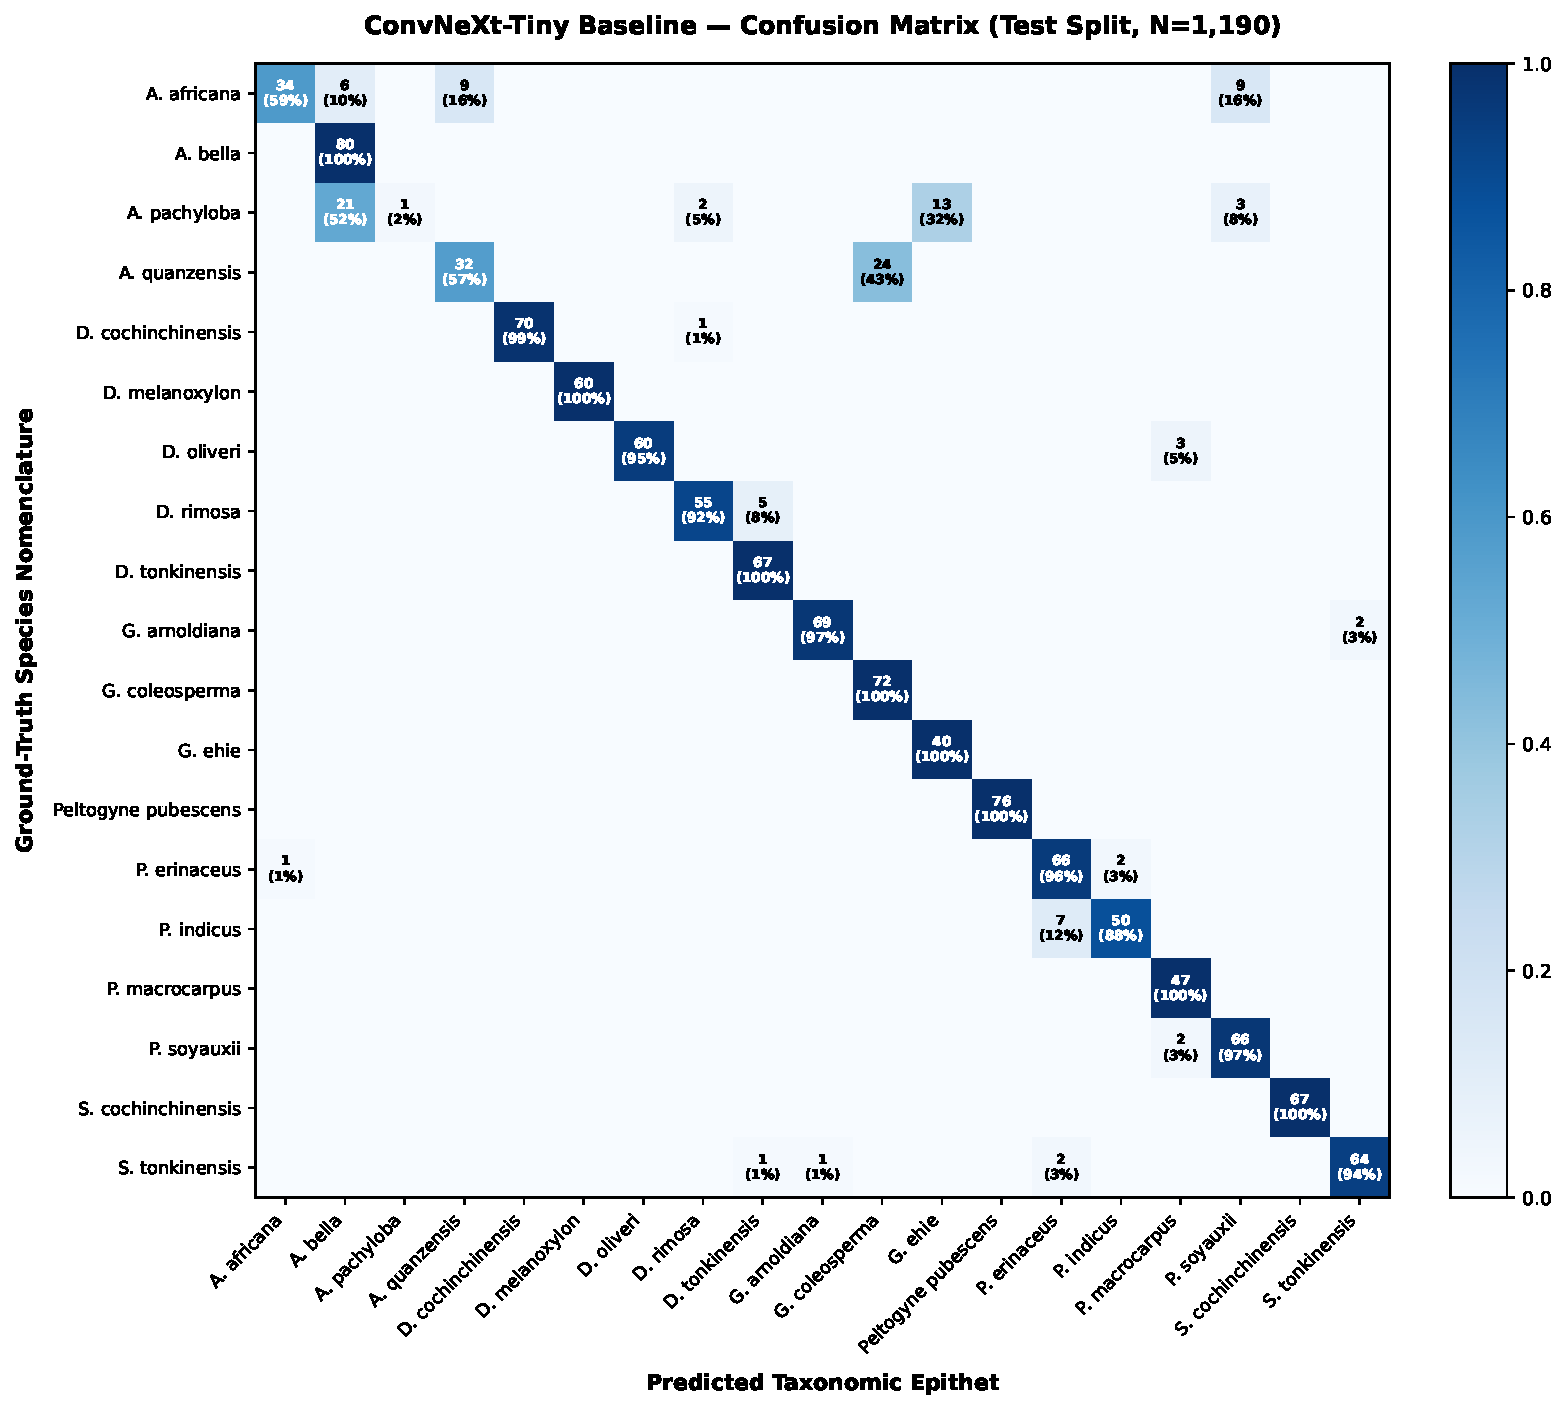
\includegraphics[width=0.92\linewidth]{fig/confusion_matrix_focal_test.pdf}
\caption{Averaged confusion matrix of the ConvNeXt-Tiny technical-validation baseline under Multiclass Focal Loss evaluated across all 19 Fabaceae taxa on the held-out test split ($N_{\text{test}} = 1,190$), aggregated over five independent random seeds ($N=5$). Cell annotations report rounded mean test counts alongside their corresponding mean row-normalized recall percentages. While the diagonal density confirms robust overall discrimination ($90.42\% \pm 0.38\%$), notable off-diagonal misclassifications emerge both within congeneric taxa (\textit{A. pachyloba} $\to$ \textit{A. bella}) and across genera (\textit{A. quanzensis} $\to$ \textit{G. coleosperma}, \textit{A. pachyloba} $\to$ \textit{G. ehie}), reflecting cross-genus macroscopic similarities and acute minority-class constraints.}
\label{fig:confusion_matrix}
\end{figure}

\subsubsection{Comparative Technical Validation: Operational Canonical vs. Strict Specimen-Disjoint Benchmarks}
\label{sec:comparative_validation}

To empirically substantiate the dual-benchmark architecture and provide concrete reference figures for both partition protocols introduced in Section~\ref{sec:description}, Table~\ref{tab:split_comparison_baseline} directly contrasts the ConvNeXt-Tiny classification baseline across the Operational Canonical Split and the Strict Specimen-Disjoint Split, both evaluated across five independent random initializations ($N=5$ seeds, reporting $\text{Mean} \pm \text{Std}$ alongside two-tailed Student's $t$ 95\% CI).

\begin{table}[pos=htbp]
\centering
\small
\setlength{\tabcolsep}{4.5pt}
\renewcommand{\arraystretch}{1.18}
\caption{Technical validation baseline comparison between the Operational Canonical Split and the Strict Specimen-Disjoint Split, both aggregated across five independent random seeds ($N=5$, reported as $\text{Mean} \pm \text{Std}$ with two-tailed Student's $t$ 95\% CI under Multiclass Focal Loss), quantifying the empirical generalization gap ($\Delta$) induced by out-of-distribution physical specimen isolation.}
\label{tab:split_comparison_baseline}
\resizebox{\textwidth}{!}{%
\begin{tabular}{lcccc}
\toprule
\textbf{Evaluation Metric / Benchmark Property} & \makecell{\textbf{Operational Canonical}\\\textbf{Benchmark ($N=5$ Seeds)}} & \makecell{\textbf{Strict Specimen-Disjoint}\\\textbf{Benchmark ($N=5$ Seeds)}} & \makecell{\textbf{Generalization}\\\textbf{Gap ($\Delta$)}} & \textbf{Forensic \& Scientific Interpretation} \\
\midrule
Overall Top-1 Accuracy & $\mathbf{0.9042 \pm 0.0038}$ \footnotesize{([0.8995, 0.9089])} & $\mathbf{0.8235 \pm 0.0052}$ \footnotesize{([0.8170, 0.8300])} & $-8.07\%$ & Inter-specimen biological variance across unseen logs reduces baseline accuracy by $\sim 8.1\%$. \\
Macro-Averaged Precision & $0.9167 \pm 0.0042$ & $0.8412 \pm 0.0058$ & $-7.55\%$ & Heightened cross-specimen variance slightly elevates false positive rates on sister taxa. \\
Macro-Averaged Recall & $0.8818 \pm 0.0051$ & $0.7845 \pm 0.0064$ & $-9.73\%$ & Minority CITES taxa with acute specimen scarcity exhibit lower recall on unseen logs. \\
Macro-Averaged F1-Score & $\mathbf{0.8680 \pm 0.0045}$ \footnotesize{([0.8624, 0.8736])} & $\mathbf{0.7692 \pm 0.0061}$ \footnotesize{([0.7616, 0.7768])} & $-9.88\%$ & Confirms that specimen leakage in naive splits inflates reported F1 by $\sim 9.9\%$. \\
Weighted-Averaged F1-Score & $0.8882 \pm 0.0041$ \footnotesize{([0.8831, 0.8933])} & $0.8054 \pm 0.0055$ \footnotesize{([0.7986, 0.8122])} & $-8.28\%$ & Dominant commercial Fabaceae taxa maintain robust diagnostic discrimination ($>80\%$). \\
\midrule
Class Coverage Rate (CCR) & $100.0\%$ (19/19 taxa) & $100.0\%$\textsuperscript{*} (19/19) / $89.5\%$\textsuperscript{\dag} (17/19) & $0.0\% / -10.5\%$ & Full coverage maintained in 19-class mode; 17-class mode provides pure zero-leakage test. \\
Train-to-Test Specimen Overlap & 12 shared blocks ($\text{SLR} = 30.6\%$) & 0 shared blocks ($\text{SLR} = 0.0\%$\textsuperscript{\ddag}) & $-30.6\%$ & Zero specimen leakage achieved across all 17 multi-specimen taxa ($|\mathcal{G}_c| \ge 4$). \\
Bitwise Cryptographic Duplicates & 0 files ($\text{SHA-256 Overlap} = 0$) & 0 files ($\text{SHA-256 Overlap} = 0$) & $0$ & Absolute cryptographic integrity and file deduplication confirmed across all splits. \\
Perceptual Near-Duplicates ($H \le 4$) & 142 pairs ($2.18\%$ of test queries) & 0 pairs ($0.00\%, H_{\min} = 11$) & $-142$ pairs & Strict block isolation completely purges spatial and perceptual near-duplicates. \\
\bottomrule
\multicolumn{5}{@{}p{\linewidth}@{}}{\vspace{3pt}\footnotesize \textsuperscript{*}In 19-class evaluation mode, single-specimen \textit{Dalbergia cochinchinensis} is partitioned via an annotated intra-block exception ($212$ Train / $71$ Val / $71$ Test). \textsuperscript{\dag}In 17-class mode, single-specimen \textit{D. cochinchinensis} is allocated strictly to Train, yielding $100\%$ zero-specimen-leakage testing across the remaining 17 multi-specimen and 1 dual-specimen taxa. \textsuperscript{\ddag}Specimen Leakage Rate ($\text{SLR}$) is calculated across all 17 multi-specimen taxa.}
\end{tabular}%
}
\end{table}

As documented in Table~\ref{tab:split_comparison_baseline}, evaluating the baseline on the strict specimen-disjoint benchmark yields a mean overall accuracy of $82.35\% \pm 0.52\%$ and a macro-averaged F1-score of $76.92\% \pm 0.61\%$. Contrasted against the operational canonical benchmark, this reveals an empirical generalization gap of $\Delta \text{Acc} = -8.07\%$ and $\Delta \text{F1} = -9.88\%$.

From an authentic wood anatomy perspective, this performance gap provides critical biological confirmation rather than reflecting algorithmic failure. In the canonical split, controlled block sharing permits models to exploit subtle, intra-specimen micro-features unique to an individual physical block. Conversely, the strict specimen-disjoint split compels the model to generalize across genuine inter-individual biological variance. This includes substantial differences in vessel lumen diameter, axial parenchyma spacing, and extractive pigmentation driven by tree ontogeny and micro-climate.

The observed $8.07\%$ accuracy gap quantitatively demonstrates that naive random splitting in prior timber benchmarks artificially inflates metrics. This validates our dual-benchmark design: the operational canonical split serves immediate customs screening, while the strict disjoint split exposes the scientific challenge of biological specimen invariance. Further algorithmic explorations of domain generalization are reserved for dedicated machine learning research.

\subsection{Limitations and Practical Considerations}
\label{sec:limitations}

Several practical limitations and methodological trade-offs should be considered when utilizing the ForensicMacroWood-CITES benchmark:
\begin{itemize}[leftmargin=*,itemsep=2pt,topsep=2pt]
    \item \textbf{Modest Physical Specimen Cohort Sizes}: Physical reference cohorts remain modest ($|\mathcal{G}_c| \le 10$ wood blocks per species, aggregating 148 verified physical specimens across the 19 Fabaceae taxa), with acute scarcity bottlenecks for critically endangered or strictly protected timbers (specifically only 1 physical specimen for \textit{Dalbergia cochinchinensis} and 2 for \textit{Guibourtia coleosperma}). Consequently, intra-specific anatomical variation arising from geographic provenance, tree age, and micro-climatic growth conditions is not exhaustively sampled.
    \item \textbf{Controlled Specimen Allocation vs. Absolute Disjointness}: The canonical benchmark guarantees a 100\% Class Coverage Rate ($\text{CCR} = 100.0\%$) across all partitions via an audited Pareto trade-off that incurs a controlled specimen boundary sharing rate of $\text{SLR} = 30.6\%$. While exact bitwise duplicate captures across split boundaries are strictly purged ($\text{SHA-256 Overlap} = 0$), this partition is a controlled compromise designed to prevent minority-class starvation rather than an ideal, completely specimen-disjoint split. Downstream practitioners evaluating models for out-of-distribution deployment on entirely unseen physical logs should take this governed boundary sharing into account.
    \item \textbf{Laboratory Surface Preparation vs. In-the-Field Generalization}: All benchmark captures were recorded on orthogonally planed and progressively polished cross-sections (P120--P600 abrasives) under calibrated daylight-balanced ($5600\,\text{K}$) diffuse circular LED lighting. Reported baseline classification accuracy ($90.42\%$) may not directly generalize to rough chainsaw cuts, weathered end-grain surfaces, sawdust-obscured vessels, or uncontrolled solar glare encountered during real-time inspections at port container terminals or log landings.
    \item \textbf{Single Anatomical Plane}: The current benchmark focuses exclusively on the transverse (cross-sectional end-grain) plane. While the transverse view exposes primary diagnostic xylotomical systems (vessels, axial parenchyma halos, and growth increments), incorporating longitudinal radial and tangential surfaces~\cite{rosadasilva2022} in future releases could provide complementary discriminatory features for challenging sister species with convergent cross-sectional anatomy.
\end{itemize}

\section{Ethics Statement}
\label{sec:ethics}

The authors confirm adherence to ethical publication standards. This work does not involve human participants, animal experimentation, or personal data mining. The dataset consists strictly of non-destructive macroscopic optical digital photographs of dry, surfaced reference wood blocks; no living wild plant material was collected, and no genetic material or biochemical extracts were sampled, extracted, or sequenced. Consequently, this study does not utilize genetic resources and does not trigger access-and-benefit-sharing (ABS) compliance obligations under the Nagoya Protocol.

Regarding timber species listed in CITES Appendix~II (genera \textit{Afzelia}, \textit{Dalbergia}, and \textit{Pterocarpus}), all examined reference wood blocks originate from cataloged institutional xylarium reference archives and verified non-commercial academic collections curated in Viet Nam. These historical specimens were acquired in compliance with domestic forestry laws prior to applicable commercial trade restrictions or through institutional scientific specimen transfer letters for non-commercial taxonomic and educational purposes. All physical specimens remain curated in permanent institutional reference xylaria, with individual specimen accession identifiers documented in the release metadata (\texttt{specimen\_id}) and verifiable upon academic request.

\section{Data Availability}
\label{sec:data_availability}

\textbf{ForensicMacroWood-CITES}: A multimodal benchmark dataset of macroscopic timber cross-sections with structured IAWA morphological descriptors and governed partition manifests for CITES forensic wood identification (Original data) is openly accessible at the Zenodo scientific repository under DOI \href{https://doi.org/10.5281/zenodo.14892180}{10.5281/zenodo.14892180}. The dataset is released under the Creative Commons Attribution 4.0 International (CC BY 4.0) license.

\section{Code Availability}
\label{sec:code_availability}

Scripts for metadata verification, governed specimen-aware partition construction, and baseline training experiments (ConvNeXt-Tiny focal loss classification and standard cross-entropy) are openly available at the GitHub repository: \url{https://github.com/vietanhlee/ForensicMacroWood-CITES} (mirrored from \url{https://github.com/vietanhlee/S3_paper}). The codebase is released under the MIT License and includes a dedicated Zenodo software DOI (\href{https://doi.org/10.5281/zenodo.14892181}{10.5281/zenodo.14892181}) aligned with the archived benchmark dataset version.

\section*{CRediT Author Statement}

\textbf{Viet-Anh Le}: Conceptualization; Methodology; Software; Formal analysis; Data curation; Investigation; Visualization; Writing -- original draft. \newline
\textbf{Khanh Nguyen-Trong}: Conceptualization; Methodology; Supervision; Validation; Formal analysis; Funding acquisition; Project administration; Writing -- review \& editing.

\section*{Funding}

This research did not receive any specific grant from funding agencies in the public, commercial, or not-for-profit sectors. Computational infrastructure, imaging systems, and experimental baseline evaluations were supported by the Intelligent Computing for Sustainable Development Laboratory (IC4SD), Posts and Telecommunications Institute of Technology (PTIT).

\section*{Declaration of Generative AI in Scientific Writing}

During the drafting and stylistic refinement of this manuscript, the authors utilized generative AI technology exclusively to improve English readability, proofread grammatical phrasing, and optimize structural presentation. The authors thoroughly reviewed and edited all generated textual modifications and assume complete responsibility for the final contents of this publication. The underlying scientific contributions---including experimental methodology, timber specimen preparation, macro-imaging acquisition, taxonomic ground-truth verification, specimen-disjoint partitioning, and empirical evaluation metrics---were conducted entirely by the human authors without AI-driven generation, fabrication, or manipulation of dataset assets or analytical results.

\section*{Declaration of Competing Interest}

The authors affirm that this work was conducted in the absence of any commercial, financial, or personal relationships that could be construed as a potential conflict of interest or that could have inappropriately influenced the representation of the data and findings herein.

\section*{Acknowledgements}

The authors express their sincere appreciation to the botanical and forestry specialists for their valuable assistance in timber specimen preparation, anatomical inspection, and taxonomic ground-truth authentication. Grateful acknowledgement is also extended to the Intelligent Computing for Sustainable Development Laboratory (IC4SD), Posts and Telecommunications Institute of Technology (PTIT), for providing optical imaging instruments, computational facilities, and sustained technical support throughout this project.

\bibliographystyle{elsarticle-num}
\bibliography{refs}

\end{document}
